\documentclass{article}
\usepackage[utf8]{inputenc}
\usepackage{amsmath}
\usepackage{amssymb}
\usepackage{titlesec}
\newcommand{\sectionbreak}{\clearpage}
\usepackage{hyperref}
\usepackage{amsthm}

\setlength{\parindent}{0pt}
\setlength{\parskip}{0.5em}

\theoremstyle{definition}
\newtheorem{defn}{Definition}[section]
\newtheorem{conj}{Conjecture}[section]
\newtheorem{exmp}{Example}[section]

\theoremstyle{plain}% default
\newtheorem{thm}{Theorem}[section]
\newtheorem{lem}[thm]{Lemma}
\newtheorem{prop}[thm]{Proposition}
\newtheorem*{cor}{Corollary}

\theoremstyle{remark}
\newtheorem*{rem}{Remark}
\newtheorem*{note}{Note}
\newtheorem*{rec}{Recall}

\newcommand{\union}{\cup}
\newcommand{\Union}{\bigcup}
\newcommand{\intersection}{\cap}
\newcommand{\Intersection}{\bigcap}

\newcommand{\injection}{\hookrightarrow}

\newcommand{\cross}{\times}

\newcommand{\R}{\mathbb{R}}
\newcommand{\Q}{\mathbb{Q}}
\newcommand{\C}{\mathbb{C}}
\newcommand{\Z}{\mathbb{Z}}

\newcommand{\interior}[1]{%
  {\kern0pt#1}^{\mathrm{o}}%
}

\usepackage{tikz}

\title{M2PM5 (metric spaces and topology) notes}
\author{Emma Tye}
\date{Spring 2019}

\begin{document}

\maketitle

\tableofcontents

% \section*{Lecture plan}

% \subsection*{Lectures 1-6}

% Metric spaces

% \begin{itemize}
%     \item  A measure of distance is assumed
%     \item Continuous functions
% \end{itemize}

% \subsection*{Lectures 7-13}

% Topological spaces

% \begin{itemize}
%     \item A measure of distance is NOT assumed
%     \item Open/closed sets
%     \item Continuous functions
% \end{itemize}

% \subsection*{Lectures 14-24}

% \begin{itemize}
%     \item Connected, compact spaces
%     \item Completeness
% \end{itemize}

% \subsection*{Lectures 25-30}

% Fundamental group of a topological space

\section{Metric spaces}

\subsection{Continuous functions}

\begin{defn}[Continuous real functions]
A function $f: \mathbb{R} \to \mathbb{R}$ is continuous at $x_0$ if $\forall \epsilon$, $\exists \delta$ such that if $|x - x_0| < \delta$ then $|f(x) - f(x_0)| < \epsilon$.
\end{defn}

\begin{defn}[Continuous vector functions]
A function $f: \mathbb{R}^n \to \mathbb{R}^m$ is continuous at $\underline{x_0}$ if $\forall \epsilon$, $\exists \delta$ such that if $||x - x_0|| < \delta$ then $||f(x) - f(x_0)|| < \epsilon$.
\end{defn}

\begin{defn}[Metric spaces]
Let $X$ be a set, and let $d$ be a function $X \times X \to \mathbb{R}$ such that the following conditions hold:
\begin{enumerate}
    \item Positivity (and 0-equality): for any $x, y \in X$, we have $d(x,y) \ge 0$ and $d(x,y) = 0$ if and only if $x=y$ 
    \item Symmetry: for any $x,y \in X$, we have $d(x,y) = d(y,x)$
    \item Triangle inequality: for any $x,y,z \in X$, we have $d(x,z) \le d(x,y) + d(y,z)$
\end{enumerate}

\begin{flushleft}
Then the pair $(X,d)$ is called a \textbf{metric space}.
\end{flushleft}
\end{defn}

\begin{rem}
We assume $X$ to be non empty.
\end{rem}

\begin{flushleft}
This essentially defines $d$ as a distance operator.
\end{flushleft}

\begin{exmp}[Vector spaces]
The Euclidean metric on $\mathbb{R}^n$:
\[d(x,y) = \sqrt{\sum_{i=1}^n (x_i - y_i)^2}\]

\begin{enumerate}
    \item Holds \checkmark
    \item Holds \checkmark
    \item Holds \checkmark
\end{enumerate}

\end{exmp}

\begin{exmp}[Function spaces] Let $X = \{\text{all continuous functions } f:[0,1] \to \mathbb{R}\}$, and define \[d_1(f,g) = \int_0^1 |f(t) - g(t)| dt\]

\begin{enumerate}
    \item Holds \checkmark
    \item Holds \checkmark
    \item Holds \checkmark
\end{enumerate}

\begin{flushleft}
We can also define \[d_2(f,g) = sup_{t \in [0,1]} |f(t)-g(t)|\] Now we have that the pair $(X, d_2)$ is also a metric space (left as exercise).
\end{flushleft}

\end{exmp}

\begin{exmp}[Discrete metric]
Let $X$ be any set, and define \[d(x,y) = \begin{cases} 0, \; (x=y) \\ 1, \; otherwise \end{cases}\]

\begin{enumerate}
    \item Holds \checkmark
    \item Holds \checkmark
    \item Holds \checkmark
\end{enumerate}

\end{exmp}

\begin{flushleft}
In an exam setting, you would prove each of the three conditions for the pair to be a metric space.
\end{flushleft}

\begin{rem}
It's important to make the metric space precise.
\end{rem}

\begin{defn}[Continuous metric functions]
Let $f$ be a map $X \to Y$ where $(X,d_x)$ and $(Y,d_y)$ are metric spaces. Then $f$ is called continuous at $x_0 \in X$ if $\forall \epsilon > 0$, $\exists \delta > 0$ such that if $d_x(x,x_0) < \delta$ then $d_y(f(x), f(x_0)) < \epsilon$.

This $f$ is called continuous if it is continuous at every point in $X$.
\end{defn}

\begin{exmp}
The functions $\mathbb{R}^2 \to \mathbb{R}$ $(x,y) \mapsto x+y$ and $(x,y) \mapsto xy$ are continuous.
\end{exmp}

\begin{prop}[Continuity preserved over composition]\label{continuity_over_comp}
Let $(X, d_x)$ $(Y,d_y)$ and $(Z,d_z)$ be metric spaces. Let $f:X \to Y$ and $g:Y \to Z$ be maps. If $f$ and $g$ are continuous, then their composition $g \circ f : X \to Z$ is also continuous.
\end{prop}

\begin{proof}
Let $x_0 \in X$. Then $\forall \epsilon$, $\exists \delta$, we have $d_y(y, f(x_0)) < \delta$ implies $d_z(g(y), g(f(x_0))) < \epsilon$. We also have that $\forall \delta$, $\exists \delta_1$, we have $d_x(x, x_0) < \delta_1$ implies $d_y(f(x), f(x_0)) < \delta$. Composing these two statements, we obtain that $g \circ f$ is continuous at $x_0$, which is arbitrary hence it is continuous everywhere.
\end{proof}

\begin{cor}
Let $(X,d)$ be a metric space, and let $f, g:X \to \mathbb{R}$ be continuous maps. Then these are all continuous maps:

\begin{itemize}
    \item $|f|$
    \item $f+g$
    \item $fg$
\end{itemize}

\begin{flushleft}
If $f:X \to \mathbb{R}\setminus\{0\}$ then $\frac{1}{f}$ is continuous.
\end{flushleft}

\end{cor}

\begin{defn}[Product of metric spaces]
Let $(X,d_x)$ and $(Y,d_y)$ be metric spaces. Then $X \times Y = \{(x,y) \, | \, x \in X, \, y \in Y\}$. Then define \[d_1((x_1,y_1), (x_2,y_2)) = d_x(x_1, x_2) + d_y(y_1,y_1)\] We have that $(X \times Y, d_1)$ is a metric space.
\end{defn}

\begin{flushleft}
\begin{itemize}
    \item The distance $d_1$ is obviously always positive as $d_x, d_y$ are always positive. And if $d_1 (...) = 0$ we also have that $x_1=x_2$ and $y_1=y_2$. \checkmark
    \item Obvious. \checkmark
    \item This also holds from summing the triangle inequalities from $d_x, d_y$. \checkmark
\end{itemize}
\end{flushleft}

\begin{rem}
There are other metric spaces for the cross product of spaces. We can define another measure of distance \[d_2((x_1, y_1), (x_2, y_2)) = \sqrt{(x_1-x_2)^2 + (y_1-y_2)^2}\] and another one as \[d_{\infty} = max(d_x(x_1,x_2), d_y(y_1,y_2))\]
\end{rem}

\begin{flushleft}
There are many more meaures. Later we will show that each of the metrics for the product of spaces give rise to the same notion of a continuous function (are in the same class).
\end{flushleft}

\begin{prop}[Product of continuous maps]
Let $f: X \to X'$ be a continuous map from metric space $(X, d_X)$ to $(X', d_X')$ and let $g : Y \to Y'$ be a continuous map from metric space $(Y, d_Y)$ to $(Y', d_Y')$. Then the map $X \times Y \to X' \times Y'$ given by $(x,y) \mapsto (f(x), g(y))$ is continuous.
\end{prop}

\begin{proof}
Fix $(x_0, y_0) \in X \times Y$.
We must show that $\forall \epsilon > 0 \exists \delta > 0$ such that if $d_1((x,y), (x_0, y_0)) < \delta$ then $d_1((f(x), g(y), (f(x_0), g(y_0))) < \epsilon$.

Fix $\epsilon < 0$.
$f$ is continuous at $x_0$ implies that $\exists \delta_1$ such that $d_X(x, x_0) < \delta_1 \implies d_{X'}(f(x), f(x_0)) < \frac{1}{2}\epsilon$. $g$ is also continuous at $y_0$ so  $\exists \delta_2$ such that $d_Y(y, y_0) < \delta_2 \implies d_{Y'}(g(y), g(y_0)) < \frac{1}{2}\epsilon$.

Take $\delta = min(\delta_1, \delta_2)$. Then if $d_1((x,y), (x_0, y_0)) < \delta$ then $d_X(x, x_0) + d_Y(y, y_0) < \delta$, hence $d_X(x, x_0) < \delta_1$ and $d_Y(y, y_0) < \delta_2$. Therefore we have that $d_{X'}(f(x), f(x_0)) < \frac{1}{2}\epsilon$ and $d_{Y'}(g(y), g(y_0)) < \frac{1}{2}\epsilon$, hence by summing we have that $d_2((f(x), g(y)), (f(x_0), g(y_0)))$.
\end{proof}

\begin{prop}[Projection map continuous]
Let $(X, d_X), (Y, d_Y)$ be metric spaces. Consider the map from $X \times Y \to X$ given by $(x,y) \mapsto x$ - called the projection to $X$. This is a continuous map.
\end{prop}

\begin{proof}
Fix $(x_0, y_0) \in X \times Y$. We have that $d_X(x, x_0) < d_1((x,y), (x_0, y_0))$. Fix $\epsilon > 0$ and take $\delta = \epsilon$. Then if $ d_1((x,y), (x_0, y_0)) < \delta$ then we have  $d_X(x, x_0) < d_1((x,y), (x_0, y_0)) < \delta = \epsilon$ so we are done.
\end{proof}

\begin{defn}[Diagonal map $\Delta$]
The diagonal map $\Delta : X \to X \times X$ is defined to be the map $x \mapsto (x,x)$ - just repeating the input $x$ for both entries.
\end{defn}

\begin{prop}[Diagonal map continuous]
Let $(X, d_X)$ be a metric space. Then $\Delta$ is continuous.
\end{prop}

\begin{proof}
Fix $x_0 \in X$. Then $d_1((x,x), (x_0,x_0)) = 2d_X(x, x_0)$. Fix $\epsilon > 0$. Let $\delta = \frac{1}{2}\epsilon$. Then if $d_X(x, x_0) < \delta$ then $d_1((x,x), (x_0,x_0)) = 2d_X(x, x_0) < 2\delta = \epsilon$.
\end{proof}

\subsection{Boundedness}

\begin{rec}
A subset $S \subset \mathbb{R}$ is bounded if $\exists C > 0$ such that $|x| < C$ for any $x \in S$.
\end{rec}

\begin{defn}[Bounded metric spaces]
A subset $S$ of a metric space $(X, d)$ is bounded if $\exists x_0 \in X$ and $\exists K > 0$ such that $d(x, x_0) \le K$ for all $x \in S$.
\end{defn}

\begin{rem}
It doesn't matter the point you choose: if this holds for some $x_0 \in X$, then this holds for any $x_0 \in X$ by the triangle inequality. Indeed, take any $x_1 \in X$. Then $d(x, x_1) \le d(x, x_0) + d(x_0, x_1) \le K + d(x_0, x_1)$. Choose $K_1 = K + d(x_0, x_1)$. Then $d(x, x_1) \le K_1$.

If $x,y \in S$ then $d(x,y) \le d(x,x_0) + d(y, x_0) \le 2K$. Hence $\sup_{x,y \in S} d(x,y)$ exists.
\end{rem}

\begin{defn}
Let $S$ be a non-empty bounded subset of a metric space $(X, d)$. Then the diameter of $S$ is defined as $diam(S) = \sup_{x,y, \in S}(d(x,y))$.
\end{defn}

\begin{defn}
A map $f$ from a set $S$ to a metric space $(X,d)$ is called bounded if $f(S)$ is a bounded set in $X$.
\end{defn}

\begin{prop}
Let $S_1, ... , S_n$ be bounded subsets of $(X,d))$. Then $\bigcup_{i=1}^n S_i$ is a bounded subset of $(X,d)$.
\end{prop}

\begin{proof}
By induction, it is enough to prove this for $n=2$.

Take $S_1, S_2$ bounded subsets of $(X,d)$. By the previous remark, we can use the same point $x_0$ for $S_1$ and $S_2$. \[d(x, x_0) \le K_1\] \[d(x, x_0 \le K_2)\] for $x \in S_1$ and $x \in S_2$ respectively. Take $K = \max(K_1, K_2)$. This works for $S_1 \cup S_2$.
\end{proof}

\subsection{Subspaces, openness and closedness}

Let $S$ be a subset of a metric space $(X,d)$. Restrict $d : X \times X \to \mathbb{R}$ to $S \times S \to \mathbb{R}$. Then all the conditions hold for $d:  S \times S \to \mathbb{R}$, so $(S,d)$ is a metric space.

\begin{exmp}
Take $\mathbb{R} \subset \mathbb{R}^2$ as the line $(x,0)$, then the restriction of the Euclidean distance is the usual distance of $\mathbb{R}$.
\end{exmp}

\subsubsection{(Open) Balls}

\begin{defn}[Open balls]
Let $(X,d)$ be a metric space. Let $x_0 \in X$ and $r \in \mathbb{R}_{\ge 0}$. The open ball in $X$ of radius $r$ centred at $x_0$ is \[B_r(x_0) = \{x \in X \; | \; d(x, x_0) < r\}\]
\end{defn}

\begin{exmp}
In $\R^2$, we can take the distance $d_1((x_1, y_1), (x_2, y_2)) = |x_1-x_2| + |y_1-y_2|$, then the ball $B_1(0,0)$ looks like a rhombus (diamond) around the origin.
\end{exmp}

\begin{exmp}
We can also take $d((x_1, y_1), (x_2, y_2)) = \sup(|x_1-x_2|, |y_1- y_2|)$. Then the ball $B_1(0,0)$ looks like a square around the origin.
\end{exmp}

\begin{exmp}
Let $X = \{f : [0,1] \to \R \; | \; f \text{ continuous }\}$ be the space of all continuous functions from the interval $[0,1]$ to the real line. Let $d(f,g) = \max_{x \in [0,1]}(||f(x) - g(x))$. Then the ball $B_1(0)$ (ball over the zero function) is \[\{f : [0,1] \to \R \; | \; \Gamma_f \subset [0,1] \times (-1, 1)\} \] \[ \{f : [0,1] \to \R \; | \; \max_{x \in [0,1]} (|f(x)|) < 1\} \] \[ \{f : [0,1] \to \R \; | \; \forall x \in [0,1] \; -1 < f(x) < 1\} \] using the extreme value theorem.
\end{exmp}

\begin{defn}
We define $\Gamma_f = \{(x,y) \in \R^2 \; | \; y = f(x))\}$ with $f : \R \to \R$.
\end{defn}

We can now restate the definition of continuous functions over metric spaces:

\begin{defn}\label{cont using balls defn}[Continuity using balls]
Take $(X, d_X), (Y, d_Y)$ metric spaces. Then $f: X \to Y$ is continuous at $x_0 \in X$ if \[\forall \epsilon >0 \; \exists \delta > 0 \; : \; f((B^X_{\delta} (x_0)) \subset B^Y_{\epsilon} (f(x_0)))\]
\end{defn}

\begin{prop}\label{open ball prop}
Let $(X, d)$ be a metric space. Fix $x \in X$ and $r \in \R_{> 0}$. Then $\forall y \in B_r(x), \; \exists \epsilon > 0$ such that $B_{\epsilon} (y) \subset B_r(x)$.
\end{prop}

This means that no matter how close you pick $y$ to the boundary of the original ball, we can still cast a ball around $y$ which is still contained inside the original ball.

\begin{proof}
Fix $x \in X, r \in \R_{> 0}$. Take arbitrary $y \in B_r(x)$. Now we can choose $\epsilon = r - d(x,y) > 0$. Take $z \in B_{\epsilon}(y)$, then $d(z,x) \le d(z,y) + d(y,x) < \epsilon + d(y,x) = r - d(x,y) + d(y,x) = r$, hence $z \in B_r(x)$.
\end{proof}

\subsubsection{Open sets}

\begin{defn}\label{open subspace defn}[Open subspace]
Let $(X,d)$ be a metric space. Then $U \subset X$ is open if \[\forall x \in U \; \exists \epsilon \; : \; B_{\epsilon}(x) \subset U\]
\end{defn}

\begin{rem}
Prop. \ref{open ball prop} says that (open) balls are open subspaces.
\end{rem}

\begin{exmp}
The interval $(a,b) \subset \R$ is open wrt definition \ref{open subspace defn}.
\end{exmp}

\begin{exmp}
Intervals $[a,b], [a,b)$ are NOT open.
\end{exmp}

\begin{prop}
A function $f : X \to Y$ is continuous if and only if $\forall U \subset Y$ then if $U$ is open $\implies \; f^{-1}U \subset X$ is open.
\end{prop}

\begin{proof}
$\rightarrow$ Suppose $f$ is continuous. Fix $U \subset Y$ open and $x \in f^{-1}(U)$. We need to prove that $exists \delta > 0$ such that $f(B_{\delta} (x)) \subset U$.

Consider $y = f(x)$. Then $\exists \epsilon > 0$ such that $B_{\epsilon}(y) \subset U$ as $U$ is open. Since $f$ is continuous $\exists \delta$ such that $f(B_{\delta}(x)) \subset B_{\epsilon}(y) \subset U$.

$\leftarrow$ Now we need to suppose that $\forall U \subset Y$ is open $\implies \; f^{-1}U \subset X$ is open. Fix $x \in X$ - we need to show that $f$ is continuous at $x$. Fix $\epsilon > 0$. By Prop \ref{open ball prop} we have that $B_{\epsilon}(f(x))$ is open. Hence $f^{-1} (B_{\epsilon}(f(x))) = V$ is open. We have that $x \in V$ and by the definition of open $\exists \delta$ such that $B_{\delta}(x) \subset V$ i.e. $f(B_{\delta}(x)) \subset B_{\epsilon}(f(x))$, which makes $f$ continuous by definition \ref{cont using balls defn}.
\end{proof}

We could say that $f : X \to Y$ is open if and only if $\forall U \in X$, if $U$ is open then $f(U)$ is open. HOWEVER: continuity does not imply openness, and openness does not imply continuity in general.

\begin{prop}\label{prop open sets}[Properties of open sets]
\hspace{0.1em}
\begin{enumerate}
    \item Suppose $U_1, U_2, ..., U_n \subset X$ are open. Then $\bigcap_{i=1}^n U_i$ is open.
    \item Let $I$ be any set. Suppose given $\forall i \in I$, $U_i \subset X$ are open, then $\Union_{i \in I}U_i \subset X$ is open.
\end{enumerate}
\end{prop}

\begin{proof}
\hspace{0.1em}
\begin{enumerate}
    \item Fix $x \in \bigcap_{i=1}^{n}U_i$. We have that $U_1$ is open: $\exists r_1$ such that $B_{r_1}(x)\subset U_1$, and we also have that for $U_2$, $\exists r_2$ such that $B_{r_2}(x) \subset U_2$. We can take the smallest of $r_1, r_2$, say $r$ such that the ball $B_r(x)$ is contained in both balls. We can repeat this process $n$ times for find the final $r$ to find the ball contained inside the intersection (i.e. the smallest $r$ over all the $U_i$).
    \item Trivial. Fix $x \in \Union_{i \in I} U_i$. Then $\exists i $ such that $x \in U_i$. Since $U_i$ is open, we can find a ball $B_r(x) \subset U_i \subset \Union_{i \in I} U_i$.
\end{enumerate}
\end{proof}

\subsubsection{Closed sets}

\begin{defn}[Closed subsets]
A subset $F \subset X$ is closed if and only if the complement $X-F$ is open.
\end{defn}

\begin{prop}[Properties of closed sets]
\hspace{0.1em}
\begin{enumerate}
    \item If we have $F_1, ... , F_n$ closed, then $\Union_{i=1}^n F_i$ is closed.
    \item Take any set $I$, and collection of $F_i$ with $i \in I$ closed. Then $\bigcap_{i \in I} F_i$ is closed.
\end{enumerate}
\end{prop}

\begin{proof}
\hspace{0.1em}
\begin{enumerate}
    \item We have that $X - (\Union_{i=1}^n) F_i = \bigcap_{i=1}^n (X - F_i)$ (i.e. the complement of unions is the intersection of the complements) - since the $F_i$ are closed their complements are open, and intersections of open sets are open.
    \item Similar.
\end{enumerate}
\end{proof}

\begin{exmp}
$[a,b] \in \R$ is closed.
\end{exmp}

\begin{defn}[Closed balls]
The closed ball $\overline{B_r(x)}$ is defined to be \[\{y \in X \; | \; d(y,x) \le r\}\]
\end{defn}

\begin{exmp}
The closed ball $\overline{B_r(x)}$ is closed.
\end{exmp}

\begin{prop}
Take any $x \in X$, $r \in \R_{>0}$, $y \in X, y \not\in \overline{B_r(x)} = \emptyset$. Then we can find $\epsilon > 0$ such that $B_{\epsilon}(y) \cap \overline{B_r(x)} = \emptyset$.
\end{prop}

\begin{defn}[Limit point]
Let $(X, d)$ be a metric space, $A \subset X$. Then $x \in X$ is a limit point of $A$ if \[\forall \epsilon > 0, \; (B_{\epsilon}(x) - \{x\} \cap A \ne \emptyset)\]
\end{defn}

\subsubsection{Closure}

\begin{defn}[Closure of subspaces]
Let $(X,d)$ be a metric space with $A \subset X$. Then the closure of $A$ is the set \[\overline{A} = \bigcap_{A \subset F \text{ closed in } X} F\]
Note: $\overline{A}$ is closed, and is the smallest closed subset that contains $A$.
\end{defn}

\begin{exmp}
Let $A \subset \R$, $A = \{\frac{1}{n} \; | \; n=1,2,3,..\}$, then the only limit point of $A$ is 0. We have that $\overline{A} = \{0\} \union A$.
\end{exmp}

\begin{prop}
The closure of $A \subset (X,d)$, $\overline{A}$, is the set $A \union \{$limit points of $A\}$.
\end{prop}


(For the time being, denote $A' = A \union \{$limit points of $A\}$)

\begin{proof}
The Proposition follows from the following lemmas \ref{lem a clos} and \ref{lem b clos}. Indeed, $\overline{A} = \bigcap_{Z \text{closed in} X, A \subset Z}Z$. By \ref{lem a clos}, $A'$ is one of these $Z$. By \ref{lem b clos}, $A'$ is contained in every closed $Z$ containing $A$. So the intersection of all the $Z$ will be equal to $A'$.
\end{proof}


\begin{lem}\label{lem a clos}
$A'$ is closed in $X$.
\end{lem}

\begin{proof}
We need to show that $U = X \setminus A'$ is open (i.e. the complement is open). Take any $x \in U$. Suppose that there is no $r$ such that $B_r(x) \subset U$. Then for any $r > 0$, $B_r(x)$ contains a point of $A'$ - either a point in $A$ or a limit point of $A$. Take $r = \frac{1}{n}$. Then $\exists a_n \in A'$ such that $d(x,a_n) < \frac{1}{n}$. If $a_n \in A$, then write $b_n = a_n$. If $a_n \not\in A$ i.e. $a_n$ is a limit point of $A$, then $\exists b_n \in A$ such that $d(a_n, b_n) < \frac{1}{n}$ by definition of a limit point. Then $d(b_n, x) \le d(x,a_n) + d(a_n, b_n) < \frac{2}{n}$. So the sequence $(b_n)$ converges to $x$. But the $b_n$ are elements of $A$ hence $x$ is a limit point of $A$ and cannot be in the complement of $A'$, so contradiction.
\end{proof}

\begin{lem}\label{lem b clos}
If $Z \subset X$ is a closed subset containing $A$, then $Z$ contains the limit points of $A$.
\end{lem}

\begin{proof}
Take $x$ to be a limit point of $A$. For a contradiction suppose that $Z \subset X$ is closed, $A \subset Z$ but $x \not\in Z$. Hence $x \in X \setminus Z$ which is an open subset of $X$. So there is some $r > 0$ such that $B_r(x) \subset X \setminus Z \subset X \setminus A$. This implies that this open ball contains no elements of $A$, however this contradicts $x$ being a limit point.
\end{proof}

\begin{defn}[Density]
A subset $A$ of a metric space $(X,d)$ is called a dense subset of $X$ if it's closure $\overline{A} = X$.
\end{defn}

\begin{exmp}
$\Q$ is dense in $\R$.
\end{exmp}

\begin{exmp}
Every subset is dense in its closure.
\end{exmp}

\begin{prop}[Properties of the closure]
Let $(X,d)$ be a metric space. Let $A,B \subset X$. Then we have the following:
\begin{enumerate}
    \item $A \subset \overline{A}$
    \item If $A \subset B$ then $\overline{A} \subset \overline{B}$
    \item If $A$ is closed then $A = \overline{A}$
    \item The closure of the closure $\overline{\overline{A}} = \overline{A}$
    \item $\overline{A}$ is the smallest closed subset of $X$ containing $A$
\end{enumerate}
\end{prop}

\begin{proof}
Trivial by inspection.
\end{proof}

\subsubsection{Interior}

\begin{defn}[Interior]
Let $A$ be a subset of the metric space $(X, d)$. The interior of $A$ is defined as the union \[\Union_{u \text{ open in } X, u \subset A} u \] denoted by $\interior{A}$.

This is also equivalent to the set of all points in $A$ of which an open ball can be cast around which is contained in $A$:\[\interior{A} = \{a \in A \; | \; \exists \epsilon > 0 \; : \; B_{\epsilon}(a) \subset A\}\]
\end{defn}

\begin{rem}
There is a "dual notion" to the closure and the interior: \[X \setminus \interior{A} = \overline{X \setminus A}\]
\end{rem}

\begin{prop}[Properties of the interior]
Let $A$ and $B$ be subsets of $(X,d)$.
\begin{enumerate}
    \item $\interior{A} \subset A$
    \item $A \subset B \implies \interior{A} \subset \interior{B}$
    \item If $A$ is open in $X$, then $\interior{A} = A$
    \item $\interior{\interior{A}} = \interior{A}$
    \item $\interior{A}$ is the largest open set contained in $A$
\end{enumerate}
\end{prop}

\begin{proof}
Left as an exercise. Can use the "dual notion" and the properties of the closure or from the naive way.
\end{proof}

\subsubsection{Boundary}

\begin{defn}[Boundary]
Let $A \subset (X,d)$. The boundary of $A$ is defined as \[\delta A = \overline{A} \setminus \interior{A}\]
\end{defn}

\begin{exmp}
Let $A = \Q$, $X = \R$ and $d$ be the usual notion of distance. Then $\overline{A} = \R$. If $x \in \interior{\Q}$, then there is a small interval centred at $x$ containing only rational numbers. This is not possible as the irrational numbers are dense in the rational numbers, so $\interior{\Q} = \emptyset$. Hence $\delta \Q = \R$.
\end{exmp}

\begin{rem}
Left as an exercise, we can also define the boundary of $A$ as \[\delta A = \{x \in X \; | \; \forall \epsilon > 0 \; : \; B_{\epsilon}(x) \text{ contains a point of } A \text{ and a point of } X \setminus A\}\]
\end{rem}

\subsection{Sequences}

\begin{defn}[Convergence]
Let $(X,d)$ be a metric space, and let $x \in X$. A sequence $(x_n)_{n=1}^{\infty}$ converges to $x$ if and only if $\forall \epsilon > 0$, $\exists N$ such that $\forall n \ge N$ we have that $x_n \in B_{\epsilon}(x)$. We write $x_n \to x$ in this case.
\end{defn}

\begin{prop}[Well-defined limits]
Let $(X,d)$ be a metric space, and $(x_n)$ be a sequence of points. Suppose that $x,y \in X$ such that $x_n \to X$ and $x_n \to Y$. Then $x=y$.
\end{prop}

\begin{proof}
Assume $x \ne y$. Then $d(x,y) \ne 0$. Take $\epsilon = \frac{1}{2} d(x,y)$. Then $B_{\epsilon}(x) \cap B_{\epsilon}(y) = \emptyset$. (Indeed, if $z \in B_{\epsilon}(x) \cap B_{\epsilon}(y)$, then $d(z,x) < \epsilon$ and $d(z,y) < \epsilon$ and $d(x,y) \le d(x,z) + d(z,y) < 2\epsilon = d(x,y)$ which is a contradiction.) By the definition of convergence, we can find an $N$ such that $\forall n \ge N$, $x_n$ is contained in $B_{\epsilon}(x)$ and also $B_{\epsilon}(y)$, hence a contradiction.
\end{proof}

\begin{prop}
Let $A \subset (X,d)$ and let $x \in X$. If there is a sequence $(a_n)$ of elements of $A$ such that $a_n \to X$, then $x \in \overline{A}$.
\end{prop}

\begin{proof}
Recall that $\overline{A} = A \union \{$limit points of $A \}$. If $x \in A$, then we are done. If $x \not\in A$ then $x$ is a limit point of $A$.
\end{proof}

\begin{cor}
A closed subset of $(X,d)$ contains all the limit points of its convergent sequences.
\end{cor}

\begin{proof}
For a closed subset $A$, we have that $\overline{A} = A$.
\end{proof}

\begin{defn}[Cauchy sequences]
A sequence $(x_n)$ in $(X,d)$ is called a Cauchy sequence if $\forall \epsilon > 0$, $\exists N$ such that $\forall n, m \ge N$ we have that $d(x_n, x_m) < \epsilon$.
\end{defn}

\begin{prop}[Cauchy is well-defined]
A convergent sequence is a Cauchy sequence.
\end{prop}

\begin{proof}
Same as real analysis, who could've guessed. Apparently an exercise. God taking this course was a good idea.
\end{proof}

\begin{note}
Now we can define convergent sequences differently for $\R^2$ using the different ball shapes of $d_1 = |x-x'| + |y-y'|$ or $d_{\infty} = \max(|x-x'|, |y-y'|)$. But it turns out that using these metrics are equivalent. However, something called the "discrete metric" is not.
\end{note}

\subsection{Equivalent spaces}

\begin{defn}[Equivalence of metrics]
Let $X$ be a set, and let $d_x$ and $d_{x'}$ be metrics on $X$. We call $d_x$ and $d_{x'}$ equivalent if $U \subset X$ is open for $d_x$ if and only if $U$ is open for $d_{x'}$, i.e. $(X,d_x)$ and $(X, d_{x'})$ give the same class of open sets.
\end{defn}

\begin{rec}
$U \subset X$ is open for $d_x$ if $\forall x \in U$, $\exists \epsilon > 0$ such that $B_{\epsilon}(x) \subset U$.
\end{rec}

\begin{exmp}
Let $X = \R^2$. Then the Euclidean distance $d_2$ casts a circle around a point, whereas $d_1$ casts a diamond around a point. However, we can fit a circle inside a diamond and a diamond inside a circle by adjusting the radius, hence the notion of open sets is the same.

Exercise is to prove that $d_{\infty} = \max(|x-x'|, |y-y'|)$ is equivalent to $d_2$.
\end{exmp}

\begin{prop}[Continuity preserved over equivalence]
Let $f : X \to Y$ be a function. Let $d_x$ and $d_{x'}$ be equivalent metrics on $X$, and let $d_y$ and $d_{y'}$ be equivalent metrics on $Y$. Then $f: (X,d_x) \to (Y,d_y)$ is continuous if and only if $f: (X, d_{x'}) \to (Y, d_{y'})$ is continuous.
\end{prop}

\begin{proof}
We previously proved that $f:X \to Y$ is continuous if for every open set $U \subset Y$, we have the pre-image $f^{-1}(U) \subset X$ is open. Since equivalent metrics preserves openness of sets by definition, the continuity of a function is also preserved across equivalent metric spaces.
\end{proof}

\section{Topological spaces}

The philosophy is that a "shape" up to a "continuous deformation", like curling a piece of paper in on itself, or moulding something into shape with no cuts, is determined in maths by the notion of a continuous map, which in turn is determined by the class of \textbf{open sets}.

\subsection{Topologies and Examples}

\begin{defn}[Topological space]
A topological space is a pair $(X, \tau)$ of a non-empty set $X$ together with a family (set) of subsets of $X$ named $\tau$, that satisfy the following axioms:
\begin{enumerate}
    \item $\emptyset \in \tau$ and $X \in \tau$
    \item If $U \in \tau$ and $V \in \tau$, then $U \cap V \in \tau$, i.e. $\tau$ is closed under intersection
    \item If $U_i \in \tau$ indexed by $i \in I$, then $\Union_{i \in I}U_i \in \tau$
\end{enumerate}

$\tau$ is called a topology on $X$, and the elements of $\tau$ are called open sets.
\end{defn}

\begin{exmp}[Discrete topology]
Let $\tau$ be the set of all subsets of $X$. Then all the axioms hold. Then $(X, \tau)$ is called the discrete topology - every subset of $X$ is open.
\end{exmp}

\begin{exmp}
Any metric space $(X,d)$ is a topological space. $\tau$ consists of the open subsets of $X$, i.e. all $U \subset X$ such that $\forall x \in U$, $\exists \epsilon > 0$ such that $B_{\epsilon}(x) \subset U$. Then, we have that the intersection of two open sets is open, and the union of indexed open sets is open, so we satisfy the axioms.
\end{exmp}

\begin{exmp}["In-discrete topology"]
Take $\tau = \{\emptyset, X\}$. Then all the axioms hold.
\end{exmp}

\begin{exmp}[Cofinite topology]
Take $X$ to be any set. Call $U \subset X$ open if $X \setminus U$ is finite (also define $\emptyset$ to be open). Then $X \setminus X = \emptyset$ is finite. 

Take $U, V \in \tau$. Then $U \cap V$ is open iff $X \setminus (U \cap V)$ is finite. $X \setminus (U \cap V) = (X \setminus U) \union (X \setminus V)$ and the union of two finite sets is finite.

Take $U_i \in \tau$. The $X \setminus (\Union_{i \in I} U_i) = \Cap_{i \in I} X \setminus U_i$ is the intersection of finite sets which is finite.
\end{exmp}

\begin{note}
The cofinite topology naturally appears in algebraic geometry. Take any field $k$. Defined closed subsets of $k$ as follows: $Z \in k$ is closed iff $\exists f(t) \in k[t]$ such that $Z = \{x \in k \; | \; f(x) = 0\}$ i.e. $Z$ is the set of all roots of a polynomial $f$ with coefficients in $k$.

Then the compliment to finite sets are declared to open. This is the simplest kind of Zariski topology.
\end{note}

\begin{prop}[Alternative definition of openness]\label{open by open neighbourhoods}
Let $X$ be a topological space. Then a subset $U \subset X$ is open if and only if $\forall x \in U$, the exists an open set $U_x$ containing $x$ such that $U_x \subset U$. Such a $U_x$ is called an open neighbourhood of $x$.
\end{prop}

\begin{proof}
$\rightarrow$ Clearly if $U$ is open, then we can take $U_x = U$ for every $x$.

$\leftarrow$ Assume that for each $x \in U$, we have an open neighbourhood $U_x$ such that $x \in U_x \subset U$. Consider $\Union_{x \in U}U_x$ - by the axioms of a topological space, this is an open set. Indeed, $U_x \subset U \implies \Union_{x \in U}U_x \subset U$. On the other hand, for any $x \in U$, $x \in U_x$ and hence $U \subset \Union_{x \in U}U_x$.
\end{proof}

\begin{defn}[Open neighbourhood]
    An open neighbourhood of $x$ is any open set containing $x$ - we usually denote such a neighbourhood $U_x$, but they are by no means unique for each $x$.
\end{defn}

\begin{defn}[Continuous functions]
Let $X,Y$ be topological spaces. Call a map $f: X \to Y$ continuous if for every open set $U \in Y$, the pre-image $f^{-1}(U)$ is open in $X$.
\end{defn}

\begin{prop}
Let $X,Y,Z$ be topological spaces, and let $f: X \to Y$ and $g : Y \to Z$ be continuous maps. The $g \circ f$ is continuous.
\end{prop}

\begin{proof}
Take any open set $U \subset Z$. Then $g^{-1}(U)$ is open in $Y$, hence $f^{-1} \circ g^{-1}(U)$ is open in $X$, so $(g \circ f)^{-1}(U)$ is open in $X$.
\end{proof}

\begin{defn}[The coarser relation]
Suppose $X$ is a set with topologies $\tau_1$ and $\tau_2$, with $\tau_1 \subset \tau_2$. $\tau_1$ is then said to be coarser than $\tau_2$, and conversely $\tau_2$ is said to be finer than $\tau_1$.
\end{defn}

\begin{exmp}
The "in-discrete" topology ($\tau = \{ \emptyset, X \}$) is coarser than every other topology. 

The discrete topology ($\tau = \mathcal{P}(X)$) is finer than every other topology. 
\end{exmp}

\begin{prop}
\begin{enumerate}
    \item Let $X$ be a topological space. Then $X \to^{\text{id}} X$ is a continuous map.
    \item Let $X, Y$ be topological spaces. Let $f : X \to Y$ be a constant map, i.e.
    \[ \exists y_0 \in Y \text{ such that } \forall x \in X, f(x) = y_0 \]
    Then $f$ is continuous.
    \item Assume $X$ has discrete topology. Then any map $f: X \to Y$ for any topological space $Y$ is continuous.
    \item Assume $Y$ has "in-discrete" topology. Then any map $f: X \to Y$ for any topological space $X$ is continuous.
\end{enumerate}
\end{prop}

\begin{proof}
\begin{enumerate}
    \item Easy.
    \item If $U \subset Y$ is an open set with $y_0 \in U$, then $f^{-1}(U) = X$ is an open set.

    If $U \subset Y$ is an open set with $y_0 \not \in U$, then $f^{-1}(U) = \emptyset$ is an open set.
    \item Easy.
    \item See that $f^{-1}(\emptyset) = \emptyset$ and $f^{-1}(Y) = X$, and these are both open. As $\emptyset, Y$ are the only open sets of $Y$, the proof of continuity is complete.
\end{enumerate}
\end{proof}

%TODO: This might not be a section
\subsection{Isometry}

\begin{defn}[Homeomorphism]
Let $X, Y$ be topological spaces. A bijection $f: X \to Y$ is a homeomorphism if both $f$ and $f^{-1}$ are continuous maps.

In particular, $U \subset X$ is open iff $f(U) \subset Y$ is open.
\end{defn}

\begin{defn}[Homeomorphic]
Let $X, Y$ be topological spaces. $X$ and $Y$ are said to be homeomorphic if there exists a homeomorphism between them.
\end{defn}

\begin{defn}[Basis]
Let $(X, \tau)$ be a topological space. A basis for $\tau$ is a subset $\beta \subset \tau$ such that any open set in $X$ (i.e. any element of $\tau$) is a union of sets from $\beta$.
\end{defn}

\begin{exmp}
Consider $\R^2$ with the Euclidean topology. Then consider $\beta = \{ B_\epsilon(x), \epsilon > 0, x \in \R^2 \}$ - this is a basis for $\R^2$.

Indeed, any open set $U \subset \R^2$ can be written as $U = \Union_{x \in U} B_{\epsilon_x}(x)$ by the definition of an open set.

Now consider $\beta' = \{ B_\epsilon(x), \epsilon \in \Q^{+}, x \in \Q^2 \}$ - this is also a basis for $\R^2$.

Indeed, if $x \in U$ is an element of an open set, we can find $a \in \Q^2$ contained in $U$ such that $x \in B_\delta(a)$, where $\delta \in \Q$. Since $\beta'$ is countable, we see that the Euclidean topology on $\R^2$ has a countable basis.
\end{exmp}

\begin{prop}
Let $f: X \to Y$ be a map. Let $\tau_X$ be a topology on $X$, and $\tau_Y$ a topology on $Y$. Let $\beta$ be a basis for $\tau_Y$ - then $f$ is continuous iff $\forall U \in \beta, f^{-1}(U)$ is open. 
\end{prop}

\begin{proof}
$\rightarrow$ This is clear by the definition of a continuous map.

$\leftarrow$ Let $U \subset Y$ be any open set. Then $U = \Union_{i \in I} U_i$, where $U_i \in B$. Then $f^{-1}(U) = \Union_{i \in I} f^{-1}(U_i)$. We know that $f^{-1}(U_i)$ is open in $X$ by assumption, hence $\Union_{i \in I}f^{-1}(U_i) = f^{-1}(U)$ is open in $X$.
\end{proof}

\begin{defn}
A topological space $(X, \tau)$ has a countable basis if $\tau$ has a countable basis $\beta$.
\end{defn}

\begin{defn}[Closed set]
Let $X$ be a topological space. A subset $V \subset X$ is closed if $X \backslash V$ is open.
\end{defn}

\begin{prop}
\begin{enumerate}
    \item $\emptyset$ and $X$ are closed.
    \item If $V_1$, $V_2$ are closed, then $V_1 \union V_2$ is closed.
    \item If $V_i$ are closed sets indexed by any set $I$, then $\Intersection_{i \in I} V_i$ is closed.
\end{enumerate}
\end{prop}

\begin{proof}
Combine the topological axioms and the use of complements.
\end{proof}

\begin{rem}
    Any metric space is a topological space, but not necessarily vice versa. In particular, consider the indiscrete topology over a set $X$ of at least two points, say $x, y$. Then $\emptyset$ and $X$ are the only open sets, and so it is not true that there exist open neighbourhoods $U_x, U_y$ about $x, y$ such that $U_x \intersection U_y = \emptyset$ - whereas in a metric space this must hold.
\end{rem}

\begin{defn}
    Let $X$ be a topological space, and take $A \subset X$. Then the closure of $A$ is \[\overline{A} = \Intersection_{A \subset V \subset X \text{ closed}} V \]
\end{defn}

\begin{rem}
    By the third property of closed sets, $\overline{A}$ is a closed subset of $X$, and furthermore it is the smallest closed subset of $X$ containing $A$.
\end{rem}

\begin{defn}[Point of closure]
    Let $X$ be a topological space, and take $A \subset X$. A point $x \in X$ is called a point of closure of $A$ if any open neighbourhood of $x$ contains a point of $A$.
\end{defn}

\begin{prop}
    \label{closure of A is points of closure}
    The closure $\overline{A}$ is the set of points of closure of $A$ in $X$.
\end{prop}

\begin{proof}
    Let $A'$ be the set of points of closure of $A$ - to show that $A' = \overline{A}$, it is enough to prove that
    \begin{enumerate}
        \item $A'$ is closed in $X$.
        \item If $A \subset V$, where $V$ is closed in $X$, then $A' \subset V$.
    \end{enumerate}
    
    Then we need to show that $U = X \backslash A'$ is open, which we do by \ref{open by open neighbourhoods}. Take $x \in U$. By the definition of $A'$, $x$ has an open neighbourhood $U_x$ such that $U_x$ doesn't contain any points of $A$. $U_x$ also doesn't contain any points of $A'$ - for a contradiction, suppose $\exists y \in A'$ such that $y in U_x$: since $y$ is a point of closure of $A$, any open neighbourhood of y, for example $U_x$, contains a point of $A$, a direct contradiction.

    Take $V$ to be a closed subset of $X$ containing $A$. Take $z \in A'$, and suppose $z \not \in V$. Then $z \in X \backslash V$, and as $X \backslash V$ is open, there is an open neighbourhood $U_z \subset X \backslash V$ with $z \in U_z$. But $X \backslash V \subset X \backslash A$, and therefore $U_z$ cannot contain any points of $A$, a contradiction of the definition of $A'$.
\end{proof}

\begin{prop}
    Let $X$ be a topological space and let $A, B \subset X$. Then
    \begin{enumerate}
        \item $A \subset \overline{A}$
        \item $A \subset B \implies \overline{A} \subset \overline{B}$
        \item If $A$ is closed, then $A = \overline{A}$
        \item $\overline{\overline{A}} = \overline{A}$
        \item $\overline{A}$ is the smallest closed subset of $X$ containing $A$.
    \end{enumerate}
\end{prop}

\begin{proof}
    Easy, use \ref{closure of A is points of closure}.
\end{proof}

\begin{defn}[Interior point]
    Let $X$ be a topological space and take $A \subset X$. A point $a \in A$ is called an interior point if there is an open neighbourhood $U_a$ such that $a \in U_a$ and $U_a \subset A$.
\end{defn}

\begin{defn}[Interior]
    The interior $\interior{A}$ is the set of interior points of $A$.
\end{defn}

\begin{rem}
    Clearly, $\interior{A} = \Union_{U \subset A \text{ open}} U$. Indeed, if $x \in \interior{A}$, then $x \in U_x \subset A$. Conversely, if $y \in \Union U$, then $y \in U$ for some $U$ open in $X$, and $U \subset A$. Then $y$ is an interior point of $A$, and $y \in \interior{A}$.
\end{rem}

\begin{prop}
    $\overline{X \backslash A} = X \backslash \interior{A}$    
\end{prop}

\begin{proof}
    \begin{align*}
         & x \not \in \interior{A} \\
        \iff & \text{there does not exist an open neighbourhood of $x$ contained in $A$} \\
        \iff & \text{every open neighbourhood of $x$ contains some point of $X \backslash A$} \\
        \iff & \text{$x$ is a point of closure of $X \backslash A$} \\
        \iff & x \in \overline{X \backslash A}
    \end{align*}
\end{proof}

\begin{prop}
    Let $X$ be a topological space and let $A, B \subset X$. Then
    \begin{enumerate}
        \item $\interior{A} \subset A$
        \item $A \subset B \implies \interior{A} \subset \interior{B}$
        \item If $A$ is open, then $A = \interior{A}$
        \item $\interior{\interior{A}} = \interior{A}$
        \item $\interior{A}$ is the largest open subset of $X$ contained in $A$.
    \end{enumerate}
\end{prop}

\begin{proof}
    Use the equivalent statements for the closure, and consider the complement.
\end{proof}

\begin{defn}
    The boundary of a subset $A$ in a topological space $X$ is $\delta A = \overline{A} \backslash \interior{A}$.
\end{defn}

\begin{rem}
    \[\delta A = \overline{A} \intersection (X \backslash \interior{A}) = \overline{A} \intersection \overline{X \backslash A}\]

    Note that the above definition is symmetric when considering $A$ or $X \backslash A$ - the two sets have the same boundary.
\end{rem}

\begin{rem}
    The notions of closure, interior, and boundary agree with the same notions for metric spaces - if we define a topology using a metric, then the definitions will agree exactly.
\end{rem}

\section{Subspaces and product spaces}

\subsection{Subspaces}

\begin{defn}[Subspace topology]
    Let $(X, \tau)$ be a topological space. Let $A \subset X$. The subspace topology $\tau_A$ is defined as 
    \[ \tau_A = \{ A \intersection U \mid U \in \tau \} \]
\end{defn}

\begin{rem}
    $(A, \tau_A)$ is a topological space. $\emptyset, A \in \tau_A$, clearly. If $U, V \subset X$ are open, then
    \[(U \intersection A) \intersection (V \intersection A) = (U \intersection V) \intersection A\]
    is open. If $U_i \subset X, i \in I$ are open, then
    \[ \Union_{i \in I} (U_i \intersection A) = (\Union_{i\in I} U_i) \intersection A \]
    is open.
\end{rem}

\begin{exmp}
    Take $[0, 1] \subset \R$. The open ball around $1$ in $\R$, restricted to $[0, 1]$, is equal to its interior - so it is open in $[0,1]$. Particularly, we must be careful that it is not open in $\R$.
\end{exmp}

\begin{defn}[Subspace]
    Let $X$ be a topological space. $A \subset X$ is a subspace of $X$ if it is a topological space equipped with the subspace topology.
\end{defn}

\begin{prop}\label{inclusion map is continuous}
    Let $X$ be a topological space and $A$ a subspace of $X$. Let $i : A \injection X$ be the inclusion map $a \mapsto a$. Then $i$ is a continuous map of topological spaces.
\end{prop}

\begin{proof}
    To show the map is continuous, we need to check that if $U$ in $X$ is open, then $i^{-1}(U)$ in $A$ is open. But $i^{-1}(U) = U \intersection A$, and by the definition of the subspace topology, this is open.
\end{proof}

\begin{cor}
    Let $f : X \to Y$ be a continuous map of topological spaces, and let $A$ be a subspace of $X$, with $i: A \injection X$ its inclusion map. Then $ f \circ i : A \to Y $ is continuous.
\end{cor}

\begin{proof}
    The composition of continuous maps is continuous.
\end{proof}

\begin{rem}
    The converse does not hold. Let $X = \R^2 \backslash \{ (a, 0) \mid a \in \R \}$, $Y = \R$, and consider the function $f : X \to Y, (a, b) \mapsto \frac{a}{b}$. Take $A \subset \R^2$ be a line i.e. $A = \{ (x, y) \mid x = ky \}$ for some fixed $k$. Then for $(x, y) \in A$, $f(x, y) = \frac{x}{y} = k$ is a constant function, and so is continuous. But $f$ is not continuous - the limit of $f$ at $(0, 0)$ depends on the direction of approach of the limit.
\end{rem}

\begin{prop}\label{inclusion continuous iff composition continuous}
    Let $i : A \injection X$ be the inclusion of a topological subspace of $A$ into the topological space $X$. Let $g : Z \to A$ be any map from a topological space $Z$ to $A$. Then $g : Z \to A$ is continuous if and only if $i \circ g : Z \to X$ is continuous.
\end{prop}

\begin{proof} $ \rightarrow $ If $g$ is continuous, then $i \circ g$ is continuous, by \ref{inclusion map is continuous}.

    $ \leftarrow $ Suppose $i \circ g : Z \to X$ is continuous. Let $U$ be any open subset of $A$. To show $g$ is continuous, we need that $g^{-1}(U)$ is open in $Z$. By the definition of the subspace topology, $\exists V \subset X$ such that $V \intersection A = U$ and $V$ is open in $X$. By the continuity of the composition, we know that $(i \circ g)^{-1}(V)$ is open in $Z$ - but $(i \circ g)^{-1}(V) = g^{-1}(i^{-1}(V)) = g^{-1}(U)$. So $g$ is continuous.
\end{proof}

\begin{rem}
    The inclusion map $i : A \injection X$ is continuous for the subspace topology, but also for many other possible topologies of $A$ - so it is not enough to characterise the subspace topology. In particular, the inclusion map is continuous for any finer topology on $A$: such as the discrete topology.
\end{rem}

\begin{prop}
    Let $X$ be a topological space, and take $A \subset A$. Let $\tau$ be some topology on $A$. Then $\tau$ is the subspace topology $\tau_A$ precisely when \ref{inclusion continuous iff composition continuous} holds, for every topological space $Z$ and every map $g: Z \to A$.
\end{prop}

\begin{proof}
    We have already shown that $\tau_A$ has the required property.

    We now assume that \ref{inclusion continuous iff composition continuous} for some topology $\tau$.

    Consider the topological space $Z = (A, \tau_A)$ and $g : A \to A$ the identity map. Then the composition of $g$ and the inclusion map of $(A, \tau)$ in $X$ is continuous, as it is equal to the inclusion map of $(A, \tau_A)$ in $X$. From the assumed property, $g$ is then a continuous map, and $\forall U \in \tau, g^{-1}(U) = U$ is an open set in $\tau_A$ - so $\tau \subset \tau_A$.

    Consider the topological space $Z = (A, \tau)$ and $g : A \to A$ the identitiy map, now with the same topology in the domain and codomain - this is continuous by definition. Then the composition of $g$ and the inclusion map of $(A, \tau)$ in $X$ is the inclusion map, and it is continuous - so $\forall U \subset X$ open, $i^{-1}(U) = U \intersection A$ is open in $\tau$ - so $\tau_A \subset \tau$.

    So $\tau = \tau_A$.
\end{proof}

\subsection{Product spaces}

Let $X$ and $Y$ be topological spaces - how could we define a topology on $X \cross Y$? We would like the topology to "agree" with the topologies on $X$ and $Y$ i.e. the projections $X \cross Y \to X$ and $X \cross Y \to Y$ to be continuous maps.

\begin{exmp}
    Let $U \subset X$ and $V \subset Y$ be open sets. We define $U \cross V$ to be open in $X \cross Y$.

    We see that this is not powerful enough - consider $X = Y = \R$. Then $X \cross Y = \R^2$, but the only possible open sets we can draw are made up of rectangles, as they are crosses of sets of open intervals. This product space does not include e.g. the open ball in $\R^2$ as an open set.
\end{exmp}

\begin{defn}
    Let $X, Y$, be topological spaces. Define $\tau$ to be the collection of all unions of the subsets of $X \cross Y$ of the form $U \cross V$ for $U$ in $X$, $V in Y$ open sets i.e. $U \times V$ form a basis for the open subsets of $X \times Y$.

    This topology on $X \cross Y$ is called the product topology.
\end{defn}

\begin{rem}
    The product topology is indeed a topology. $\emptyset = \emptyset \cross \emptyset \in \tau$ and $X \cross Y \in \tau$.

    As the sets of the topology are unions of crosses of open sets, then any union of sets in the topology is simply the union of their constituent crosses of open sets - so any union on open sets is open.

    Let $A = \Union_{i \in I} U_i \cross V_i$ and $B = \Union_{j \in J} U_j \cross V_j$. Then
    \[\left(\Union_{i\ \in } U_i \cross V_i\right) \intersection \left( \Union_{j \in J} U_j \cross V_j \right) = \Union_{i \in I} \Union_{j \in J} \left( (U_i \cross V_i) \intersection (U_j \cross V_j) \right) = \Union_{i \in I}\Union_{j \in J} \left( (U_i \intersection U_j) \cross (V_i \intersection V_j) \right) \]
    and as $U_i \intersection U_j$ is open in $X$, and $V_i \intersection V_j$ is open in $Y$, the union is open in $X \cross Y$.
\end{rem}

We see that open sets of the form $U \cross V$ for $U \subset X$, $V \subset Y$ open, form a basis for the product topology.

\begin{rem}
    A subset $W \subset X \cross Y$ is open if and only if for any $(x, y) \in W$ there exists an open subset $U \subset X$ with $x \in U$ and an open subset $V \in Y$ with $y \in V$ such that $U \cross V \subset W$. 
\end{rem}

\begin{prop}[Projection map continuous]
    The projection $p_x : X \times Y \to X$ sending $(x,y) \mapsto x$ is continuous when $X \times Y$ is given by the product topology.
\end{prop}

\begin{proof}
    Left as an exercise.
\end{proof}

\begin{prop}\label{func cont. if proj continuous prop}
    Let $X,Y,Z$ be topological spaces, and let $f$ be a map from $Z \to X \times Y$. Then $f$ is continuous if and only if $p_x \circ f$ and $p_y \circ f$ (the respective projection maps of $X \times Y$) are both continuous.
\end{prop}

\begin{proof}
    Left as an exercise.
\end{proof}

\begin{defn}[Commutative diagrams]
    Take sets $X,Y,Z,W$ and maps $X \to^f Y \to^g Z$ and $X \to^\alpha W \to^\beta Z$. If $g \circ f = \beta \circ \alpha$, then the following diagram is commutative:
    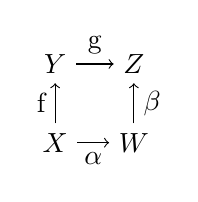
\begin{tikzpicture}
        \path (0, 0) node(x) {$X$} (0, 1) node(y) {$Y$} (1, 0) node(w) {$W$} (1, 1) node(z) {$Z$};
        \draw[->] (x) -- node[left] {f} (y);
        \draw[->] (x) -- node[below] {$\alpha$} (w);
        \draw[->] (y) -- node[above] {g} (z);
        \draw[->] (w) -- node[right] {$\beta$} (z);
    \end{tikzpicture}
\end{defn}

\begin{prop}
    Let $f : X \to X'$ and $g : Y \to Y'$ be continuous maps (on $X,X',Y,Y'$ topological spaces). Then the map $(f,g) : X \times Y \to X' \times Y'$ is continuous.
\end{prop}

\begin{proof}
    We can project $X \times Y$ to $X$ using $p_x$ and then apply $f$ to get a continuous map. Similarly for $p_y$ and $g$ - by definition we have that $p_x \circ (f,g) = f \circ p_x$ and that $p_y \circ (f,g) = f \circ p_y$. Using proposition \ref{func cont. if proj continuous prop} we have that $(f,g)$ is continuous.
    
    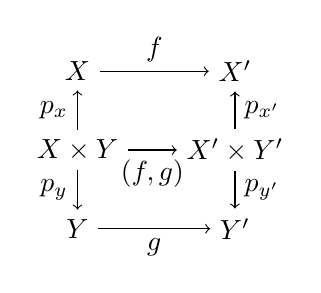
\begin{tikzpicture}
    \path (0, 0) node(xy) {$X \cross Y$} (2, 0) node(x'y') {$X' \cross Y'$} (0, 1) node(x) {$X$} (2, 1) node(x') {$X'$} (0, -1) node(y) {$Y$} (2, -1) node(y') {$Y'$};
    \draw[->] (xy) -- node[below] {$(f, g)$} (x'y');
    \draw[->] (xy) -- node[left] {$p_x$} (x);
    \draw[->] (xy) -- node[left] {$p_y$} (y);
    \draw[->] (x) -- node[above] {$f$} (x');
    \draw[->] (x'y') -- node[right] {$p_{x'}$} (x');
    \draw[->] (y) -- node[below] {$g$} (y');
    \draw[->] (x'y') -- node[right] {$p_{y'}$} (y');
    \end{tikzpicture}
\end{proof}

\begin{defn}[Diagonal map continuous]
    Let $X$ be a topological space and $\Delta : X \to X \times X$ be the diagonal map sending $x \mapsto (x,x)$. For any topology on $X$ and the respective product topology on $X \times X$, this map is continuous.
\end{defn}

\begin{proof}[Proof 1]
It is enough to check that $\Delta^{-1} (U \times V)$ is open - $(U \times V) \cap \Delta(X) = \Delta(U \cap V)$ so $\Delta^{-1}(U \times V) = U \cap V$ which is open in a topological space.
\end{proof}

\begin{proof}[Proof 2]
    Using the commutative map way, let $p_1, p_2$ be the projections of the 1st and 2nd $x$. Then $p_1 \circ \Delta = p_2 \circ \Delta = id$, and the identity map is continuous.
\end{proof}

\begin{cor}
    If $f,g$ are continuous maps from $X \to \R$, then $fg, f+g, |f|,...$ are continuous, and if $f : X \to \R \setminus \{0\}$ then $\frac{1}{f}$ is continuous.
\end{cor}

\begin{proof}
    Take $X \to^\Delta X \times X \to^{(f,g)} \R \times \R \to^+ \R$ - the last one is well-known to be continuous. Similar proofs for the other maps.
    
    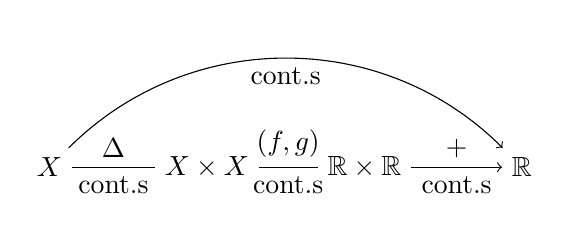
\begin{tikzpicture}
        \path (0, 0) node(x) {$X$} (2, 0) node(xx) {$X \cross X$} (4, 0) node(rr) {$\R \cross \R$} (6, 0) node(r) {$\R$};
        \draw[->] (x) -> node[above] {$\Delta$} node[below] {cont.s} (xx) -> node[above]  {$(f, g)$} node[below] {cont.s} (rr) -> node[above] {$+$} node[below] {cont.s} (r);
        \draw[->] (x) to[out=45, in=135] node[below] {cont.s} (r);
    \end{tikzpicture}
\end{proof}

\section{Hausdorff spaces}

\subsection{Convergence}

\begin{defn}[Convergence in topological spaces]
    Let $(X, \tau)$ be a topological space. Let $(x_n)$ be a sequence of elements in $X$. Let $x \in X$. We say that $(x_n) \to x$ if any open neighbourhood of $x \in X$ contains all but finitely many points of $(x_n)$.
    
    Equivalently, $\forall U_x, \exists N$ such that $\forall n \ge N$, we have $x_n \in U_x$.
\end{defn}

\begin{exmp}
    If $(X, \tau)$ comes from a metric, then this is the usual definition (since open balls form a basis for the open sets of $X$).
\end{exmp}

\begin{exmp}
    Let $(X, \tau)$ be a set $X$ with discrete topology - i.e. every subset is open. Then $\{x\}$ is an open neighbourhood of $x$. Thus $(x_n) \to x$ if and only if $\exists N$ such that $\forall n \ge N$ we have $x_n = x$.
\end{exmp}

\begin{exmp}
    Let $(X, \tau)$ be a set with indiscrete topology - the only open sets are $X, \emptyset$. Then $X$ is the unique non-empty open set. This means that any sequence $(x_n)$ converges to every point $x$. This problem comes from the fact that open sets don't separate points - we can't exclude any points.
\end{exmp}

\subsection{Hausdorff spaces}

\begin{defn}[Hausdorff spaces]
    A topological space $(X, \tau)$ is Hausdorff if for any $x,y \in X$ with $x \ne Y$, there is an open neighbourhood $U_x$ of $x$ and $U_y$ of $y$ which are disjoint i.e. $U_x \cap U_y = \emptyset$.
\end{defn}

\begin{prop}
    In a Hausdorff space, any convergent sequence has a unique limit.
\end{prop}

\begin{proof}
    For a contradiction, suppose $(x_n) \to x$, $(x_n) \to y$ with $(x \ne y)$. Then take $U_x$, $U_y$ disjoint. Then by the definition of convergence we have that only finitely many points of $(x_n)$ can be in either neighbourhood but this contradicts the infinite nature of the sequence.
\end{proof}

\begin{rem}
    Every metric space is Hausdorff. Say $x \ne y$, then $d(x,y) \ne 0$, then let $n = \frac{d(x,y)}{2}$ and $B_z(x) \cap B_z(y) = \emptyset$. Therefore a non-Hausdorff topological space cannot have a metric
\end{rem}

\begin{exmp}
    The indiscrete topology is not Hausdorff.
\end{exmp}

\begin{exmp}
    Let $X$ be an infinite set. Let $\tau$ on $X$ be the cofinite topology - closed sets only contain finitely many points (or the whole set). So open sets are the complements to finitely many points, or finite subsets of $X$. Hence if $U,V \subset X$ are non-empty open sets, then $U \cap V \ne \emptyset$ - any two finite sets have some (infintely many) points that are not in either set.
\end{exmp}

Can we characterise topological spaces which come from metric spaces?

\begin{rem}
    Points in a topological space $(X, \tau)$ are not always closed (the closure of it is itself).
\end{rem}

\begin{exmp}
    Sierpinski space: $X = \{0,1\}$ and $\tau = \{\emptyset, X, \{1\}\}$. So the closed sets are $\{\emptyset, X, \{0\}\}$. So 0 is a closed point but 1 is not.
\end{exmp}

\begin{prop}[Properties of Hausdorff spaces]
    If $(X, \tau)$ is a Hausdorff space, then for any $x \in X$ we have
    \begin{enumerate}
        \item $\Intersection_{\text{open}} U_x = \{x\}$
        \item $\{x\}$ is a closed subset of $X$
    \end{enumerate}
\end{prop}

\begin{prop}\label{Diagonal close in Haus}
    $X$ is Hausdorff if and only if $\Delta(X) \subset X \times X$ is a closed subset of $X \times X$ (in the product topology).
\end{prop}

\begin{proof}
    $(X \times X) \setminus \Delta(X)$ is open if and only if $\forall (x,y) \in X \times X$, with $x \ne y$, there is an open neighbourhood of the form $U \times V$, where $U$ is an open neighbourhood of $x$ and $V$ is an open neighbourhood of $y$, contained in $X \times X \setminus \Delta(X)$. $U \times V \subset X \times X \setminus \Delta(X)$ precisely when $U \intersection V = \emptyset$.
\end{proof}

\subsection{Hierarchy of separatedness}

\begin{defn}[Hierarchy of "separatedness" conditions]
    Let $(X, \tau)$ be a topological space.
    \begin{itemize}
        \item $T_0:$
        
        for all $x,y x \ne y$ one of $x,y$ has an open neighbourhood not containing the other point.
        \item $T_1:$
        
        for all $x,y$, $x \ne y$ both of $x,y$ have an open neighbourhood not containing the other point.
        \item $T_2:$
        
        for all $x,y$, $x \ne y$ both of $x,y$ have an open neighbourhood $U_x, U_y$ with $U_x \intersection U_y = \emptyset$.
        \item $T_3:$
        
        for any closed subset $V \subset X$, and any $x \not\in V$, there are open sets $U_V \subset X$ (such that $V \subset U_V$) and $U_x$ (such that $x \in U_x$) such that $U_V \intersection U_x$
        \item $T_4:$
        
        for any closed subsets $V, W \subset X$ with $V \intersection W = \emptyset$, then there exists $U_V, U_W$ open in $X$ such that $V \subset U_V$, $W \subset U_W$ and $U_V \intersection U_W = \emptyset$.
    \end{itemize}
\end{defn}

\begin{exmp}
    Hausdorff spaces satisfy $T_2$ and above.
\end{exmp}

\begin{prop}
    Every metric space has property $T_3$.
\end{prop}

\begin{proof}
    Let $d_X$ be a metric on $X$. Consider $a = \inf_{y \in V} d_X(x,y)$.
    \begin{itemize}
        \item $a > 0$
        
            Then we observe that by the triangle equality that $\forall y \in V$ we have $B_{\frac{a}{2}}(x) \intersection B_{\frac{a}{2}}(y) = \emptyset$. Otherwise, $z \in B_{\frac{a}{2}}(x) \intersection B_{\frac{a}{2}}(y)$ so we have that $d_X(x,y) \le d_X(x,z) + d_X(y,z) < \frac{a}{2} + \frac{a}{2} = a$. Take $U_V = \Union_{y \in V} B_{\frac{a}{2}} (y)$, $U_x = B_{\frac{a}{2}} (x)$.
        \item $a=0$
        
            This never happens!
            
            If $a = 0$, then $\forall \epsilon > 0$. there exists $y \in V$ such that $d_X(x,y) < \epsilon$ so $x$ is a point of closure for $V$, but since $V$ is closed, $x \in V$ which is a contradiction. 
    \end{itemize}
\end{proof}

\begin{prop}
    Every metric space has property $T_4$.
\end{prop}

\begin{proof}
    Take $V,W \subset X$ closed subsets with $V \intersection W = \emptyset$. For $x \in V$ define $a_x = \inf_{y \in W} d_X(x,y)$. Since $x \not\in W$, by the previous proof we have that $a_x$ is positive. Define $U_V = \Union_{x \in V} B_{\frac{a_x}{2}}(x)$. This is open and contains $V$. Take everything similarly for $W$ - $b_y = \inf_{x \in V} d_X(x,y)$. Then we take $U_W = \Union_{y \in W} B_{\frac{b_y}{2}}(y)$. All we need to prove is that $U_V \intersection U_W = \emptyset$.
    
    Assume $z \in U_V \intersection U_W$. Then $d_X(x,y) \le d_X(x,z) + d_X(y,z) < \frac{a_x}{2} + \frac{b_y}{2} \le \max(a_x, b_y)$. However, since we took the infimum of $a_x, b_y$ we have that $d_X(x,y) \ge \max(a_x,b_y)$ hence we have that $\max(a_x,b_y) < \max(a_x,b_y)$ and that is a contradiction.
\end{proof}

\begin{thm}[Urysohn]
    Let $(X,\tau)$ be a topological space with a countable basis. Then the topology $\tau$ on $X$ is given by a metric if and only if $(X, \tau)$ satisfies properties $T_1$ and $T_4$.
    
    This is non-examinable.
\end{thm}

\begin{rem}
    Can replace $T_4$ by $T_3$.
\end{rem}

\begin{prop}[Combinations of Hausdorff spaces]
    \hspace{0.1em}
    \begin{enumerate}
        \item A subspace of a Hausdorff space is Hausdorff
        \item If $f:X \to Y$ is an injective continuous map of topological spaces and $Y$ is Hausdorff, then $X$ is Hausdorff
        \item If $X,Y$ are homeomorphic topological spaces, then $X$ is Hausdorff if and only if $Y$ is Hausdorff
        \item $X \times Y$ is Hausdorff if and only if $X$ and $Y$ are both Hausdorff
    \end{enumerate}
\end{prop}

\begin{proof}
    \hspace{0.1em}
    \begin{enumerate}
        \item Let $A \subset X$. If $a,b \in X$ then there are $U_x, U_y$ are disjoint. Take an open neighbourhood of $a,b$ in $A$ - these are subsets of their respective neighbourhoods in $X$, so are also disjoint.
        \item We have that $Y$ is Hausdorff. Pick any $x,y \in X$ with $x \ne y$. Then $f(x) \ne f(y)$. There exist $U_1, U_2$ open in $Y$ such that they are neighbourhoods of $f(x), f(y)$ respectively. Since $f$ is continuous, $f^{-1}(U_1), f^{-1}(U_2)$ are open subsets of $X$ which contain $x$ and $y$ (again, respectively) which are disjoint (since $U_1,U_2$ are disjoint and $f$ is injective).
        \item $\exists f : X \to Y$ which is a bijection, and $f$ and $f^{-1}$ are continuous (from definition of homeomorphic spaces). From 2, we have that $X$ is Hausdorff if $Y$ is Hausdorff using $f$ as the injective function, and we also have that $Y$ is Hausdorff if $X$ is Hausdorff using $f^{-1}$ as the injective function.
        \item
        $\impliedby$
        
        Assume $X,Y$ are Hausdorff. We need to show that if $(x_1,y_1) \ne (x_2, y_2)$ are distinct points in $X \times Y$, then we can separate them by open neighbourhoods. WLOG assume that $x_1 \ne x_2$. Then $\exists U_1, U_2$ open in $X$ with $x_1 \in U_1$, $x_2 \in U_2$ such that $U_1 \intersection U_2 = \emptyset$. Consider $U_2 \times Y$ and $U_1 \times Y$ - these subsets are open in $X \times Y$ by definition. There are no common points between them, otherwise the $x$-coordiantes would also be in common.
        
        $\implies$
        
        Assume $X \times Y$ is Hausdorff. Consider $f_{y_0}: X \to X \times Y$,  with $x \mapsto (x, y_0)$. This map is obviously injective and continuous using the product topology - take open subset $U \times V$, then $f^{-1}(U \times V) = U$ if $y_0 \in V$, otherwise $f^{-1}(U \times V) = \emptyset$. Apply 2 to $f$ - $f$ is continuous and injective, $X \times Y$ is Hausdorff so $X$ is Hausdorff. Use similar argument for $Y$.
    \end{enumerate}
\end{proof}

\begin{prop}\label{set of agreed points is closed}
    Let $X,Y$ be topological spaces. Let $f: X \to Y$ and $g: X \to Y$ be continuous maps. Assume $Y$ is Hausdorff. Then $\{x \in X \;|\; f(x) = g(x)\}$ is a closed subset of $X$.
\end{prop}

\begin{proof}
    Take the map $(f,g) : X \to Y \times Y$ which sends $x \mapsto (f(x), g(x))$. Then $f = p_1 \circ (f,g)$ and $g = p_2 \circ (f,g)$ using the projection maps commutative diagrams. 
    
    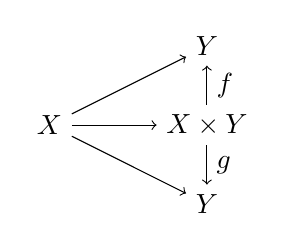
\begin{tikzpicture}
        \path (0, 0) node(x) {$X$} (2, 0) node(xy) {$X \cross Y$} (2, 1) node(fy) {$Y$} (2, -1) node(gy) {$Y$};
        \draw[->] (x) -- (xy);
        \draw[->] (x) -- (fy);
        \draw[->] (x) -- (gy);
        \draw[->] (xy) -- node[right] {$f$} (fy);
        \draw[->] (xy) -- node[right] {$g$} (gy);
    \end{tikzpicture}
    
    We know that the continuity of $p_1 \circ (f,g)$, $p_2 \circ (f,g)$ imply that $(f,g)$ is continuous. Let $S = (f,g)^{-1}(\Delta(Y))$ be the reverse image of the diagonal - this is the same as $\{x \in X \;|\; f(x) = g(x)\}$.
    Since $Y$ is Hausdorff, we know that $\Delta(Y)$ is closed in $Y \times Y$ from Proposition \ref{Diagonal close in Haus}. A map is continuous if and only if the reverse images of every open set is open, which is equivalent to the condition that the reverse images of closed sets are closed (by taking complements). Hence, since $(f,g)$ is continuous, we know that $(f,g)^{-1}(\Delta(X))$ is also closed.
\end{proof}

\begin{cor}
    Let $f: X \to X$ be continuous map, where $X$ is Hausdorff. Then the set of fixed points of $f$, $\{x \in X \; | \; x = f(x)\}$ is a closed subset of $X$.
\end{cor}

\begin{proof}
    Use the proposition, taking $g = id$.
\end{proof}

\begin{defn}[Graph of a function]
    If $f:X \to Y$ is a map of sets, then the graph of $f$ is the subset of $X \times Y$ consisting of the points $(x, f(x))$.
\end{defn}

\begin{cor}
    Let $f : X \to Y$ be a continuous map of topological spaces, with $Y$ Hausdorff. Then the graph of $f$, $\{(x,y) \in X \times Y\; | \; y = f(x)\}$ is closed.
\end{cor}

\begin{proof}
    We have two maps from $X \cross Y \to Y$ - the projection $p_Y$, which is continuous, and the composition of $f$ and the projection $p_X$, which is also continuous. As $Y$ is Hausdorff, we can apply \ref{set of agreed points is closed} on these continuous maps, but this set is equal to the graph set of $f$. So the graph is closed.
\end{proof}

\section{Connected and path-connected spaces}

\subsection{Connectedness}

\begin{defn}[Connected space]
    A topological space $X$ is connected if there is NO surjective, continuous map from $X \to \{0,1\}$, which is equipped with the discrete topology.
\end{defn}

\begin{prop}[Other ways to define connectedness]
    The following statements are equivalent:
    \begin{enumerate}
        \item $X$ is connected
        \item There do not exist two non-empty, OPEN subsets $U, V$ in $X$ such that $X = U \union V$ and $U \intersection V = \emptyset$.
        \item There do not exist two non-empty, CLOSED subsets $U, V$ in $X$ such that $X = U \union V$ and $U \intersection V = \emptyset$.
        \item The only subsets of $X$ that are simultaneously open and closed are $X$ and $\emptyset$.
    \end{enumerate}
\end{prop}

\begin{proof}
    $X$ not connected $\implies$ $\exists \; f : X \to \{1,0\}$ with the discrete topology. Then take $U=f^{-1}(0)$ and $V = f^{-1}(1)$. Then as $f$ is surjective, they are non-empty, since $f$ is continuous they are open, and they are obviously disjoint, so 1 $\implies$ 2. Conversely, if $X=U\union V$, with $U \intersection V$, then take $f(U) = \{0\}$ and $f(V) = \{1\}$. So $2 \implies 1$, hence $1 \Leftrightarrow 2$.
    
    Clearly, $2 \Leftrightarrow 3$.
    
    If 4 is false, then $X$ contains a non-empty proper subset $U$ which is open and closed. Then $X \setminus U$ is open and closed as well, so we can write $X = U \union (X \setminus U)$ which is a union of disjoint open subsets (and closed subsets), so $4 \Leftrightarrow 3$ and $4 \Leftrightarrow 2$.
\end{proof}

\begin{exmp}
    Key examples of connected spaces are $\R$, $\R^n$ and $[0,1]$.
\end{exmp}

An interval in $\R$ is a subset of one of the following types:
\begin{itemize}
    \item $(a,b)$
    \item $[a,b]$
    \item $[a,b)$
    \item $(a,b]$
\end{itemize}
with $a,b \in \R$ or $a = -\infty$ or $b = \infty$, with $[-\infty, b) = (-\infty, b)$ and same for $\infty$. $\R = (-\infty, \infty).$

\begin{prop}
    $[0,1]$ is connected.
\end{prop}

First we need a lemma to prove this:

\begin{lem}\label{Interval definition lemma}
    A non-empty subset $S \subset \R$ is an interval if and only if it has the following property: whenever $x,y \in S$ (let $x < y$ WLOG), we also have $z \in S$ for all $z$ such that $x < z < y$.
\end{lem}

\begin{proof}[Proof of lemma]
    Assume that $x,y \in S \implies (x,y) \subset S$. Define $a = \inf(S)$ and $b = \sup(S)$. $S = \Union_{\substack{x \in S \\ y \in S \\ x < y}} (x,y)$. For any $z \in S$ with $z \ne a, b$ $\exists x,y \in S$ such that $z \in (x,y)$, otherwise $z$ would be the $\sup(S)/\inf(S)$. The RHS is equal tp $(a,b)$. Thus, $S$ is an interval $(a,b), [a,b], [a,b)$ or $(a,b]$.
\end{proof}

\begin{proof}[1st proof of proposition]
    Recall that $[0,1]$ has the subspace topology from $\R$. Assume for a contradiction that $[0,1] = U \union V$ where $U,V$ are non-empty, disjoint and open in $[0,1]$. Pick $a \in U$, $b \in V$ and WLOG assume $a < b$. Hence $[a,b] \subset [0,1]$. Let $U' = [a,b] \intersection U$, $V' = [a,b] \intersection V$. Then $U'$ is closed in $[a,b]$, but $[a,b]$ is closed in $\R$ so $U'$ is closed in $\R$ - indeed, $U$ is also closed since it is the complement to $V$ which is open, and the intersection of two closed subsets in closed. Similarly, $V'$ is also closed.
    
    Define $c = \sup(U')$, so $a \le c$. Now $c$ is a limit point of $U'$, but $U'$ is closed in $\R$, $c \in U'$. In particular, $c < b$, because $b \not\in U'$. But since $U'$ is an open subset of $[a,b]$, a small neighbourhood of $c$ is contained in $U'$. Thus, $\exists \epsilon > 0$ such that $[a,b] \intersection [c,c+\epsilon] \ne \emptyset$ and $[c, c+ \epsilon] \subset U'$. This is a contradiction, because $c = \sup(U')$.
\end{proof}

\begin{proof}[2nd proof of proposition]
    For a contradiction, assume $\exists g: [0,1] \to \{0,1\}$ that is continuous and surjective. Combine it with the natural inclusion (identity) of $\{0,1\}$ into $[0,1]$, which is continuous, to get the continuous function \[f : [0,1] \; \left(\to \{0,1\}\right) \; \to [0,1]\] But by the Intermediate Value Theorem, $\exists z_0 \in [0,1]$ such that $z_0 \mapsto \frac{1}{2} \in [0,1]$, which is false and a contradiction.
\end{proof}

\begin{rem}
    The same proof(s) give that any interval is connected.
\end{rem}

\begin{prop}
    Any connected subset of $\R$ equipped with the subspace topology is an interval.
\end{prop}

\begin{proof}
    Suppose $S \subset \R$ is not an interval. By Lemma \ref{Interval definition lemma}, $S$ does not satisfy the property: $x,y \in S \; \implies \; (x,y) \subset S$. If $S = \{a\},$ then $S=[a,a]$, so $S$ must contain more than one element. So we can find $x,y \in S$, $x \ne y$ such that $(x,y) \in S$ contains $z \not\in S$. Then $S = \left(S \intersection (-\infty, z) \right) \union \left( S \intersection (z, +\infty) \right)$. But both of the intersections are open in $S$ by the subspace topology, and they are non-empty since one contains $x$ and the other contains $y$, so this is a contradiction.
\end{proof}

\begin{exmp}
    Any set $X$ with the indiscrete topology is connected (there are no other open (and closed) sets other than $X, \emptyset$).
\end{exmp}

\begin{exmp}
    Any set with more than 1 point, equipped with the discrete topology, is not connected.
\end{exmp}

\begin{exmp}
    $\Q \subset \R$ is not connected (as a subspace topology).
\end{exmp}

\begin{exmp}
    Consider the following subset $S \subset \R^2$ : \[S = \{(0,0)\} \union \left\{x, \sin \left(\frac{1}{x}\right) \; | \; x \in \R, x > 0\right\}\] Then $S$ is connected (left as an exercise).
\end{exmp}

\begin{prop}[Maps on connected spaces]\label{Maps on connected spaces}
    Let $f:X \to Y$ be a continuous map of topological spaces. If $X$ is connected, then the image $f(X)$ is connected.
\end{prop}

\begin{proof}
    Decompose $f$ into $f_1: X \to f(X)$ and $i : f(X) \to Y$ be the natural inclusion. Since $f = i \circ f_1$ is continuous, we know that $f_1$ is continuous ($i$ is obviously continuous). So WLOG we can concentrate on $f_1 : X \to f(X)$ and forget about the whole of $Y$.
    
    If $f(X)$ is not connected, then $f(X) = U \union V$ with $U,V$ open, disjoint and non-empty. Then $X = f^{-1}(U) \union f^{-1}(V)$ since $f_1$ is surjective, with $f^{-1}(U), f^{-1}(V)$ non-empty, open and disjoint which is a contradiction.
\end{proof}

\begin{cor}
    If $X$ and $Y$ are homeomorphic topological spaces, then $X$ is connected if and only if $Y$ is connected.
\end{cor}

\begin{lem}
    Let $X$ be a topological space. Let $A_i, i \in I$ be a family of connected subsets. If $A_i \intersection A_j \ne \emptyset$ whenever $i \ne j$, then $Union_{i \in I} A_j$ is connected.
\end{lem}

\begin{proof}
    Suppose $f : \Union_{i \in I} A_i \to \{0,1\}$ is continuous. We need to prove this is not surjective. Since $A_i$ is connected, $f|_{A_i}$ is a constant function. Take $i_0 \in I$. Then $f(A_{i_0})$ is 0 or 1 - WLOG say the image is 0. But then $f(A_i) = 0$ $\forall i \in I$, since the intersection of $A_i, A_{i_0}$ is non-empty, so one point in $A_i$ must map to 0 - therefore the whole subset maps to 0. Hence, $f$ is not surjective.
\end{proof}

\begin{lem}
    Suppose $X$ is a topological space with a connected subset $B \ne \emptyset$ and connected subsets $C_i$ with $i \in I$, such that $B \intersection C_i \ne \emptyset$. Then $B \union \Union_{i \in I} C_i$ is connected.
\end{lem}

\begin{proof}
    Define $A_i = B \union C_i$. By the previous lemma, $A_i$ is connected. We also have that $B \ne \emptyset$ and $B \subset A_i \intersection A_j$, so then $\Union_{i \in I} B \union C_i = B \union \Union_{i \in I} C_i$ is connected.
\end{proof}

\begin{thm}
    $X, Y$ are connected topological spaces if and only if $X \times Y$ is connected.
\end{thm}

\begin{proof}
    $\impliedby$ Let $X \times Y$ be connected. Then $p_1 : X \times Y \to X$ is continuous so that $X = p_1(X \times Y)$ is connected (the image of any connected space under a continuous function is continuous). Similar for $Y$.
    
    \begin{tikzpicture}
        \path (4, 0) node(X) {$X$} (0, 4) node(Y) {$Y$} (0, 3) node(y0) {$y_0$} (1, 0) node (x1) {$x$} (1.5, 0) node(x2) {$x$} (2.5, 0) node(x3) {$x$}; 
        \draw (y0) -- +(4, 0) node[right] {$B$};
        \draw (x1) -- +(0, 4) node[above] {$C_x$};
        \draw (x2) -- +(0, 4) node[above] {$C_x$};
        \draw (x3) -- +(0, 4) node[above] {$C_x$};
    \end{tikzpicture}
    
    $\implies$ Let $X, Y$ be connected. Fix $y_0 \in Y$. Consider the map $X \to X \times Y$ sending $x$ to $(x, y_0)$. This map is continuous (obviously, can check if you really want to). Since $X$ is connected, we know that $X \times y_0$ is a connected subspace of $X \times Y$. The same argument shows that $x \times Y$ is a connected subspace of $X \times Y$ for any $x \in X$. Now apply the previous lemas with $B = X \times y_0$ and $C_x = x \times Y$, indexed by $x \in X$. We have that $B \intersection C_x \ne \emptyset$. But $X \times Y = \Union_{x \in X} x \times Y$, so we are done.
\end{proof}

\subsection{Path-connectedness}

\begin{defn}[Paths]
    A path in $X$ is a continuous map $f: [0,1] \to X$. $f(0)$ is the beginning of the path and $f(1)$ is the end.
\end{defn}

\begin{defn}[Path-connected]
    A topological space $X$ is called path-connected if for any $x,y \in X$ there is a path $f: [0,1] \to X$ such that $f(0) = x$ and $f(1) = y$.
\end{defn}

\begin{exmp}
    Let $f$ be the constant function. Then each point is path-connected to itself.
\end{exmp}

\begin{prop}
    If a topological space $X$ is path-connected, then it is connected.
\end{prop}

\begin{proof}
    Suppose otherwise - $X$ is disconnected. Then $X = U \union V$, where $U,V$ are open, non-empty and disjoint. Choose $x \in U$ and $y \in V$. Since $X$ is path-connected, then $\exists f: [0,1] \to X$ such that $f(0) = x$ and $f(1) = y$. The interval $[0,1]$ is connected, and from Proposition \ref{Maps on connected spaces}, the image $f([0,1])$ is connected. But $f([0,1]) = \left( f([0,1]) \intersection U \right) \union \left( f([0,1]) \intersection V \right)$, and both sides of the union are open in $f([0,1])$, with both non-empty (containing $x$ and $y$ respectively). Then this is a connected open subspace, but is also the disjoint union of two open, non-empty subsets, hence a contradiction.
\end{proof}

\begin{exmp}
    $\R^n$ is path-connected.
\end{exmp}

\begin{exmp}
    Any convex subset of $\R^n$ is path-connected.
\end{exmp}

\begin{exmp}
    A circle $S^1$ (i.e. a 1-dimensional sphere) is path-connected.
\end{exmp}

\subsection{Composing paths}

\begin{defn}[Composition of paths]
    Let $f: [0,1] \to X$ and $g: [0,1] \to X$ be continuous maps, such that $f(1) = g(0)$. Define the composition as follows: \[h(t) \begin{cases} f(2t) &t \in [0, \frac{1}{2}] \\ g(2t - 1) &t \in [\frac{1}{2}, 1] \end{cases}\]
    This is well-defined, as $f(2t) = g(2t-1)$ when $t = \frac{1}{2}$ from the condition above.
\end{defn}

\begin{prop}
    The composition of paths is a continuous map $h : [0,1] \to X$.
\end{prop}

\begin{proof}
    $h(t)$ is continuous at $t \in [0,\frac{1}{2})$ from continuity of $f$, and is continuous in $(\frac{1}{2}, 1]$ from continuity of $g$. But $h(t)$ is also continuous at $t = \frac{1}{2}$ since the limits from either side converge to the same limit.
\end{proof}

\begin{prop}
    If $X$ is an open, connected, non-empty subset of $\R^n$, then $X$ is also path-connected.
\end{prop}

\begin{proof}
    Let $x \in X$. Let $U$ be the set of all points of $X$ that can be connected to $x$ by some path: i.e. $U = \{y \in X \; | : \exists f : [0,1] \to X\ \; f(0) = x, \; f(1) = y \}$.
    
    Claim: $U$ is open in $X$. Let $y \in U$. Since $X$ is open, $\exists \epsilon > 0$ such that $B_\epsilon (y) \subset X$. Let $z \in B_\epsilon (y)$, then $\exists g : [0,1] \to B_\epsilon (y)$ be continuous, sending $0 \mapsto y$ and $1 \mapsto z$. Define $h$ to be the composition of $f$ and $g$, so $z \in U$ and hence $U$ is open.
    
    If $U = X$, then we are done.
    
    For a contradiction, assume $U \ne X$. Then we can find a point $w \in X \setminus U$. Let $V_w$ be the set of all points of $X$ that can be connected to $w$ by some path. The same argument shows that $V$ is open. Take the union of all $V_w$, indexed by $w \in X \setminus U$. Then $\Union_w V_w$ is open. But $X = U \union \Union_w V_w$, which are now two open, non-empty sets. They are also disjoint - if there was a common point, $y$, then you can connect a path from $x$ to $y$ and then $y$ to $w$ so $x$ has a path to $w$, which cannot happen. Therefore, $X$ cannot be connected, which is a contradiction.
\end{proof}

\begin{rem}
    "$x$ connected to $y$ by a continuous path" is an equivalence relation:
    \begin{itemize}
        \item Clearly, $x$ is connected to itself through the constant function $f : [0,1] \to X$.
        \item If $x ~ y$, then $y ~ x$ by $f(1-t)$.
        \item If $x ~ y$ and $y ~ z$, then by composition, we have $x ~ z$.
    \end{itemize}
    
    The equivalence classes of this form are called connected components of $X$.
\end{rem}

Fundamental problem of topology: given topological spaces $X$ and $Y$, decide if they are homeomorphic or not (topologically indistinguishable).

\begin{exmp}
    Let $X = \R$ and $Y = \R^2$. They are not homeomorphic. Suppose $f: \R \to \R^2$ is a bijective continuous function with $f^{-1}$ also continuous. Then restrict $f$ to $f : \R \setminus \{0\} \to \R^2 \setminus \{f(0,0)\}$. Then $\R \setminus \{0\}$ is not connected, but $\R^2 \setminus \{f(0)\}$ is still connected (think of a graph with a point taken out). Hence, the restriction is not a homeomorphism so $f$ is not homeomorphic.
\end{exmp}

\section{Compact spaces}

\subsection{Compactness}

\begin{defn}
    A subset $C$ of $\R^n$ is called compact if it is closed and bounded.
\end{defn}

\begin{thm}
    If $C$ is a compact subset of $\R^n$, then every continuous function $f : C \to \R$ on $C$ is bounded and achieves a minimum and maximum on $C$.
\end{thm}

This definition of compact sets generalises immediately to metric spaces, but not to topological spaces - boundedness doesn't make sense in an arbitrary topological space. We want a definition that makes sense for all topological spaces, and gives rise to similar nice properties for continuous maps, and which is equivalent to the original definition when restricted to metric spaces.

\begin{defn}[Cover]
    Let $X$ be any set. A cover of $X$ is a set of subsets $U_i$ of $X$, $\{U_i, i \in I\}$, where  $\Union_{i \in I} U_i = X$.
\end{defn}

\begin{defn}[Subcover]
    A subcover of a cover $\{U_i, i \in I\}$ of $X$ is a subset $\{U_j, j \in J\}$ of the cover, for some $J \subset I$, such that $\{U_j, j \in J\}$ is still a cover of $X$, that is $X = \Union_{j \in J} U_j$.
    
    This means that our original cover contained some redundant subsets that cover $X$.
    
    A subcover is called finite if it consists of finitely many sets - that is, $J$ is finite.
\end{defn}

\begin{defn}[Open cover]
    An open cover $\{U_i, i \in I\}$ of a topological space $X$ is a cover of $X$ consisting only of open sets: each $U_i$ in the cover is open in $X$.
\end{defn}

\begin{defn}[Compactness]
    A topological space $X$ is called compact if every open cover of $X$ has a finite subcover.
\end{defn}

This property expressed that $X$ is "not too large".

\begin{exmp}
    The open interval $(0,1)$ is not compact.
    
    For every $n \ge 1$ consider the open subset $(0,1 - \frac{1}{n})$. Then $\{(0, 1- \frac{1}{n}), n \ge 1\}$ is an open cover of $(0,1)$, because $\forall x \in (0,1)$ we can find a value of $n \ge 1$ such that $0 < x < 1-\frac{1}{n}$.
    
    But this cover does not have a finite subcover. Assume that there is a finite subcover: there exists finitely many $n_1, ...., n_l$ such that $(0,1) = \Union_{1}^{i=l} (0, 1- \frac{1}{i})$. This is absurd, because $1 - \frac{1}{\max(n_1, ..., n_l) + 1}$ is still a member of $(0,1)$, but is not contained in any of the subintervals we picked, so this subcover does not cover all of $(0,1)$.
    
    The closed interval $[0,1]$ is compact - proof later.
\end{exmp}

\begin{exmp}
    If $X$ is finite with any topology, then $X$ is compact.
\end{exmp}

\begin{prop}
    Let $(X,d)$ be a metric space. Then every compact subspace $C$ of $X$ is bounded.
\end{prop}

\begin{proof}
    If $C = \emptyset$ then there is nothing to prove. Otherwise, choose any point $c \in C$ and consider the open cover $\{B_n(c), n \ge 1\}$ of $X$. Then $\{B_n(C) \intersection C, n \ge 1\}$ is an open cover of $C$, by definition of the subspace topology. Since $C$ is compact, this open cover has a finite subcover. Since the balls are nested inside each other, we only need one ball, hence when $n$ is sufficiently large, $B_n(c) \intersection C = C$. Therefore, $C \subset B_n(c)$ which is precisely the definition of boundedness. 
\end{proof}

\begin{thm}
    Let $X$ be a Hausdorff topological space (e.g. a metric space). Then every compact subspace $C \subset X$ is closed in $X$.
\end{thm}

\begin{proof}
    We want to show the complement is open i.e. $\forall x \in X \setminus C$, there exists an open neighbourhood of $x$ in $X$ that is disjoint from $C$.
    
    Choose $x \in X \setminus C$. By definition of Hausdorff spaces, for all $c \in C$ we can find open neighbourhoods of $x$ ($U_x(c)$) and of $c$ ($U_c$) that are disjoiont. Now we let $c$ run through $C$. Then $\{U_c, c \in C\}$ is a set of open sets in $X$ where $C \subset \Union_{c \in C} U_c$, since all $U_c$ contain $c$. Thus $\{U_c \intersection C, c \in C\}$ is an open cover of $C$ in $C$. By compactness of $C$, this open cover has a finite subcover $\{U_{c_1} \intersection C, ..., U_{c_n} \intersection C\}$ for some $c_1, ..., c_n \in C$. Now set $U = U_{x}(c_1) \intersection ...  \intersection U_{x}(c_n)$ is the finite intersection of open sets so is an open neighbourhood of $x$. By construction, it is disjoint from $U_{c_1} \union ... \union U_{c_n} \supseteq C$, and we are done.
\end{proof}

\begin{rem}
    If we omit that Hausdorff property, this theorem is false: if $X$ is finite, then every subspace is compact, but they are not all closed unless the topology on $X$ is discrete. 
\end{rem}

\begin{prop}
    Let $f : X \to Y$ be a continuous map of topological spaces. If $C$ is a compact subsapce of $X$, then the image $f(C)$ is a compact subspace of $Y$.
\end{prop}

\begin{proof}
    On a problem sheet.
\end{proof}

\begin{cor}
    Compactness is preserved over homeomorphisms: if $X$ and $Y$ are homeomorphic topological spaces, then $X$ is compact if and only if $Y$ is compact.
\end{cor}

\begin{cor}\label{cor metirc maps}
    Let $X$ be a compact topological space and let $(Y,d)$ be a metric space. Let $f : X \to Y$ be a continuous map. Then the image $f(X)$ if bounded and closed in $Y$. 
\end{cor}

\begin{cor}
    Let $C$ be a compact topological space and let $f : C \to \R$ be a continuous map. Then $f$ is bounded, and $f$ achieves a minimum and maximum on $C$.
\end{cor}

\begin{proof}
    By Corollary \ref{cor metirc maps}, $f(C)$ is bounded and closed in $\R$. By completeness of $\R$, $f(C)$ has a supremum and an infimum. These are limit points of $f(C)$. But since $f(C)$ is closed, it contains all of its limit points, so the supremum = maximum and infimum = minimum, which it achieves.
\end{proof}

\begin{prop}
    Every closed subspace of a compact topological space is compact.
\end{prop}

\begin{proof}
    Let $X$ be a compact topological space, and $C$ a closed subspace. Let $\{U_i, i \in I\}$ be an open cover of $C$. By the definition of the subspace topology, we can write each $U_i$ as $C \intersection V_i$ for some $V_i \subset X$ open. Since $C$ is closed, $X \setminus C$ is open, so $\{X \setminus C\} \union \{V_i, i \in I\}$ is an open cover of $X$ (both $C$ and $X \setminus C$ are covered). By compactness of $X$, there exists a finite subset $J \subset I$ such that $\{X \setminus C\} \union \{V_j, j \in J\}$ cover $X$. But then $\{U_j, j \in J\}$ cover $C$ which is a finite subcover of our original cover, hence $C$ is compact.
\end{proof}

\begin{prop}[Inverse function theorem]
    Let $X,Y$ be topological spaces and let $f: X \to Y$ be a continuous bijection. If $X$ is compact and $Y$ is Hausdorff, then $f$ is a homeomorphism.
\end{prop}

Idea: you need enough open subsets for the Hausdorff property, but you can't have too many if you want your space to be compact.

\begin{proof}
    All we need to check is that $f^{-1}$ is continuous i.e. if $C \subset X$ is closed then $(f^{-1})^{-1}(C) = f(C)$ is closed in $Y$.
    
    Since $X$ is compact and $C$ is closed, we have that $C$ is compact, therefore we know that $f(C)$ is compact. Since $Y$ is Hausdorff, any compact subspace of $Y$ is closed, hence $f(C)$ is closed.
\end{proof}

\begin{rem}
    \begin{enumerate}
        \item Suppose $X = \{0,1\}$ with discrete topology, and $Y = \{0,1\}$ with indiscrete topology. Take $f = id$. $f$ is bijective, and $f$ is continuous since $Y$ is indiscrete, but $f^{-1}$ is not continuous ($X$ is compact, but $Y$ is not Hausdorff).
        \item Suppose $X = [0,1)$, $Y = S^1$ (the unit circle - $z \in \mathbb{C}$ with $|z| = 1$), and $f(x) = e^{2\pi i . x}$. Then $f: X \to Y$ is continuous and bijective, but $f^{-1}$ is not continuous, as points very close on the circle can have values near 0 or 1. Here, $Y$ is Hausdorff but $X$ is not compact.
    \end{enumerate}
\end{rem}

\begin{thm}[Product theorem]
    If $X,Y$ are topological spaces, then $X \times Y$ is compact if and only if $X$ and $Y$ are compact.
\end{thm}

\begin{proof}
    \begin{itemize}
        \item $\impliedby$
        
        Assume that $X \times Y$ is compact. Consider the projection maps $p_x : X\times Y \to X$ and $p_y : X \times Y \to Y$ - by their definitions they're are continuous. It follows that $p_x(X \times Y) = X$ is compact, and $p_y(X \times Y) = Y$ is compact, since $X \times Y$ is compact.
        \item $\implies$
        
        Assume $X, Y$ are compact. We will prove that $X \times Y$ is compact. Let $\{W_i, i \in I\}$ be an open cover of $X \times Y$.
        
        Choose $x \in X$. Then the subspace $\{x\} \times Y$ of $X \times Y$ is homeomorphic to $Y$. Thus $\{x\}\times Y$ is compact. For every $y \in Y$, we can choose an index $i(y)$ in $I$ such that $(x,y) \in W_i(y)$ in the open cover of $X \times Y$. By the definition of the product topology on $X \times Y$, we can find an open neighbourhood $U_{x(y)}$ of $x$ in $X$ and an open neighbourhood $V_y$ of $y$ in $Y$ such that $(x,y) \in U_{x(y)} \times V_y \subset W_{i(y)}$. If we let $y$ run through $Y$, then the open sets $\{V_y, y \in Y\}$ form an open cover of $Y$. By compactness of $Y$, there exist finitely many points $y_1, ..., y_n \in Y$ such that $V_{y_1}, ..., V_{y_n}$ cover $Y$. So we can define $U_{x} = \Intersection_{i=1}^n U_{x(y_i)}$. $U_x$ is open in $X$ and $x \in U_x$, so $U_x \times Y = \Union_{i=1}^n U_x \times V_{y_i} \subseteq \Union_{j = 1}^n W_{i(y_j)}$.
        
        So the open set $U_x \times Y$ is covered by finitely many $W_i$ of our original cover.
        
        Then $\Union_{x \in X} U_x$ cover $X$, hence we can take a finite subset of this cover $U_1, ..., U_m$. Then $X \times Y = \Union U_{i} \times Y$. By the previous step, each $U_i \times Y$ is covered by finitely many $W_i$, so $X \times Y$ is covered by finitely many ($n \times m$) $W_i$s, and we are done.
    \end{itemize}
\end{proof}

\begin{rem}
    A compact subspace of a metric space is closed and bounded, but the converse is not always true: take $(0,1)$ - this is a closed, bounded subspace but not compact (as previously proved).
    
    However, the converse is true for $\R^n$.
\end{rem}

\begin{thm}[Heine-Borel]
    A subset of $\R^n$ with the subspace topology is compact if and only if it is closed and bounded.
\end{thm}


\begin{proof}[Proof of Heine-Borel theorem]
    We have that a compact set is closed and bounded since $\R^n$ is Hausdorff.
    
    So all we need is to show a closed and bounded subset is compact.
    
    Take $[0,1] \subset \R$. Let's show this is compact. Take an open cover of $[0,1]$ $\{U_i, i \in I\}$ with $U_i$ open in $\R$. Define $S = \{x \in [0,1] : [0,x] \text{ is covered by finitely many } U_i\}$. Clearly, $S$ is non-empty as $0 \in S$. Let $c = \sup S \le 1$. Assume $c < 1$. Then $\exists U_i$ such that $c \in U_i$ and $\epsilon > 0$ such that $(c-\epsilon, c+\epsilon) \subset U_i$ (cannot happen if $c = 1)$. As $c$ is the supremum, $\exists y \in S$ such that $y > c -\epsilon$ and $y \le c$. By definition of $S$, $[0,y]$ is covered by finitely many $U_i$s, say $[0,y] \subset \Union_{j \in J} U_j$ where $J$ is finite. But then $[0, c + \frac{1}{2}\epsilon] \subset \Union_{j=1} U_j \union U_i$ and so $c + \frac{1}{2}\epsilon \in S$, which is a contradiction. Hence $c = 1 = \sup(S)$. Therefore, there is a finite covering of $[0,1]$.
    
    Let $C \subset \R^n$ be closed and bounded. Then $\exists N$ such that $C \subseteq [-N, N]^n$. $[-N, N]$ is homeomorphic to $[0,1]$ so it is compact. And by the product theorem, $[-N,N]^n$ is compact in $\R^n$. Hence $C$ is a closed subset of a compact set, hence it is compact.
\end{proof}

\subsection{Another approach to compactness}

\begin{rec}
    Bolzano-Weierstrass theorem says that any bounded sequence of real numbers has a convergent subsequence.
\end{rec}

\begin{defn}[Sequentially compact]
    A metric space $(X,d)$ is called sequentially compact if any sequence of elements of $X$ has a convergent subsequence to a point of $X$.
\end{defn}

\begin{rem}
    A subset $X \subset \R$ is compact if and only if it is sequentially compact.
\end{rem}

\begin{proof}
    A compact subset $X$ of $\R$ is bounded and closed - therefore, every sequence of $X$ contains a convergent subsequence to some $a \in \R$ by Bolzano-Weierstass, but since $X$ is closed, $a \in X$.
    
    Assume every sequence of $X$ has a convergent subsequence to a point of $X$. By Heine-Borel, it is enough to prove that $X$ is bounded and closed. If $X$ is not bounded, it will contain a sequence tending to either $\pm \infty$, which does not contain a convergent subsequence, hence $X$ must be bounded. Similarly, if $X$ is not closed, then there is $a \in \overline{X} \setminus X$, therefore we can find a sequence converging to $a$, hence every subsequence converges to $a$, but then $a$ must lie in $X$.
\end{proof}

In fact, this equivalence holds for arbitrary metric spaces.

\begin{thm}
    Let $(X,d)$ be a metric space. Then $X$ is compact if and only if it is sequentially compact.
\end{thm}

\begin{lem}
    Let $(x_n)$ be a sequence of elements in $(X,d)$. If $x \in X$ is such that for each $\epsilon > 0$, $\{x_n\} \intersection B_\epsilon(x)$ is infinite, then $(x_n)$ has a subsequence converging to $x$.
\end{lem}

\begin{proof}
    Take $\epsilon = 1$. Then $\exists n_1 \in \mathbb{N}$ such that $x_{n_1} \in B_1(x)$. Take $\epsilon = \frac{1}{2}$. Then $\exists n_2 > n_1$ such that $x_{n_2} \in B_{\frac{1}{2}}(x)$. Continue by indcuction, and so obtain a subsequence $x_{n_r}$ satisfying the condition that $x_{n_r} \in B_{\frac{1}{r}}(x)$ for any $r \in \mathbb{N}$. Clearly, this subsequence converges to $x$. 
\end{proof}

\begin{proof}[Proof of theorem $\implies$]
    Assume $X$ is compact. Let $(x_n)$ be any sequence of elements of $X$. For a contradiction, suppose that for any $x \in X$, the sequence $(x_n)$ has no subsequence converging to $x$. Then $\exists \epsilon_x  > 0$ such that $(x_n) \intersection B_{\epsilon_x}(x)$ is finite by the previous lemma. The open balls $B_{\epsilon_x}(x)$ form a open cover of $X$. It has a finite subcover consisting of the open balls $B_{\epsilon_{x_1}}(x_1), ..., B_{\epsilon_{x_m}}(x_m)$. Hence, there are only finitely many terms of the sequence $(x_n)$ contained in finitely many open balls, which is a contradiction of the infinite sequence $(x_n)$.
\end{proof}

We'll now introduce a so-called "Lebesgue number" of a cover.

If we have the interval $[0,1]$, with the open covering of $U = [0, \frac{3}{4})$ and $V = (\frac{1}{4}, 1]$, then $\forall x \in [0,1]$, we have that $B_{\frac{1}{4}}(x) \subset U$ or $B_{\frac{1}{4}}(x) \subset V$. Then $\frac{1}{4}$ is a Lebesgue number.

\begin{defn}[Lebesgue number]
    Let $U_i$, $i \in I$, be a cover of a metric space $(X,d)$. A number $\epsilon > 0$ is called a Lesbesgue number for this covering if for any $x \in X$, $\exists i \in I$ such that $B_{\epsilon}(x) \subset U_i$.
\end{defn}

\begin{lem}\label{Existence of Lebesgue}
    Let $(X,d)$ be a sequentially compact metric space. Then any open cover of $X$ has a Lebesgue number.
\end{lem}

\begin{proof}
    Assume otherwise. Then there is an open cover $U_i$, $i \in I$, which has no Lebesgue number. In particular, $\frac{1}{n}$ is not a Lebesgue number for any $n$. Then $\exists x_n \in X$ such that $B_{\frac{1}{n}}(x_n) \not \subset U_i$ for any $i \in I$. We are given that $X$ is sequentially compact, so by definition, we can find a subsequence of $(x_n)$, say $(x_{n_r})$ that converges to a point $x \in X$. Let $U_i$ be an open set of the original cover such that $x \in U_i$. As $U_i$ is open, $\exists \epsilon > 0$ such that $B_{2\epsilon}(x) \subset U_i$. Since $x_{n_r} \to x$, $\exists R \in \mathbb{N}$ such that $\forall r \ge R$ we have that $d(x, x_{n_r}) < \epsilon$. But by the triangle inequality, $B_{\epsilon}(x_{n_r}) \subset U_i$. Indeed, if $y \in B_\epsilon (x_{n_r})$, then $d(y, x_r) < \epsilon$, so $d(x,y \le d(x, x_{n_r})) + d(y, x_{n_r}) = 2\epsilon$, so $y \in B_{2\epsilon}(x) \subset U_i$. Take $r$ large enough so that $\frac{1}{n_r} < \epsilon$. Then clearly $B_{\frac{1}{n_r}}(x_{n_r}) \subset B_{\epsilon}(x_{n_r}) \subset U_i$, hence a contradiction.
\end{proof}

\begin{lem}\label{Epsilon-net}
    Let $(X, d)$ be a sequentially compact metric space. Then for any $\epsilon > 0$, we can find a finite subset $A \subset X$ such that $X = \Union_{a \in A} B_{\epsilon}(a)$. Such a subset is called an $\epsilon$-net.
\end{lem}

\begin{proof}
    Suppose we have $\epsilon > 0$ for which an $\epsilon$-net $A$ doesn't exist. Take any element $x_1 \in X$. Since $\{x_1\}$ is not an $\epsilon$-net, $B_\epsilon(x_1) \ne X$. So $\exists x_2 \in X \setminus B_\epsilon(x_1)$. We have $d(x_1, x_2) > \epsilon$. Now $\{x_1, x_2\}$ is also not an $\epsilon$-net, so $\exists x_3 \in  \setminus (B_\epsilon(x_1) \union B_\epsilon(x_2))$. By induction, we construct a sequence $(x_n)$ such that $d(x_i, x_j) \ge \epsilon$ $\forall i \ne j$. So we have constructed an infinite, non-Cauchy sequence, and any subsequence will have the same property on non-Cauchy-ness - so it is not convergent, which is a contradiction.
\end{proof}

\begin{proof}[Proof of theorem $\impliedby$]
    Assume $(X,d)$ is sequentially compact. Need to prove that $X$ is compact. Let $U_i$, $i \in I$, be an open cover. By Lemma \ref{Existence of Lebesgue}, this cover has a Lebesgue number, say $\epsilon > 0$. Then by Lemma \ref{Epsilon-net}, $\exists x_1, ..., x_n \in X$ such that $X = \Union_{j=1}^n B_\epsilon(x_j)$. Since $\epsilon$ is a Lebesgue number, each $B_\epsilon(x_j)$ is contained in some $U_i$ of the original open cover. This gives a finite subcover.
\end{proof}

\subsection{Uniform continuity}

\begin{defn}[Uniformly continuous]
    Let $f: (X, d_x) \to (Y, d_y)$ be a map of metric spaces. Then $f$ is called uniformly continuous if $\forall \epsilon > 0$, $\exists \delta > 0$ such that $f(B_{\delta}(x)) \subset B_\epsilon(f(x))$.
    
    Equivalently, $\forall \epsilon > 0$, $\delta > 0$ such that if $d_x(x, x') < \delta$ then $d_y(f(x), f(x'))< \epsilon$.
\end{defn}

\begin{rem}
    $f$ is continuous if $\delta$ depends on $\epsilon$ and $x$.
    
    $f$ is uniformly continuous if $\delta$ depends only on $\epsilon$.
\end{rem}

\begin{prop}
    Let $f: (X, d_x) \to (Y, d_y)$ be a continuous map. If $X$ is compact, then $f$ is uniformly continuous.
\end{prop}

\begin{proof}
    $f$ continuous means that $\forall \epsilon$, $\exists \delta_x > 0$ such that $f(B_{\delta_x}(x)) \subset B_{\frac{\epsilon}{2}}(f(x))$. Visibly, the open balls $B_{\delta_x}(x)$ for all $x \in X$ form an open cover of $X$. By Lemma \ref{Existence of Lebesgue}, since compact is the same as sequentially compact for metric spaces, this cover has a Lebesgue number - $\delta > 0$. This means that for any $t \in X$, we have that $B_{\delta}(t) \subset B_{\delta_x}(X)$. Equivalently, for any $t, t' \in X$ such that $d_X(t, t') < \delta$, we have that $t$ and $t'$ are inside $B_{\delta_x}(x)$ for some $x \in X$. Therefore, $d_Y(f(t), f(t')) \le d_Y(f(t), f(x)) + d_Y(f(t'), f(x)) < \frac{\epsilon}{2} + \frac{\epsilon}{2} < \epsilon$.
\end{proof}

\subsection{Convergence of function}

A naive approach is pointwise convergence of a function.

\begin{defn}[Pointwise convergence of real functions]
    Take $f_n : \R \to \R$. Then $f_n \to f$ pointwise if $\forall x$, $f_n(x) \to f(x)$
\end{defn}

\begin{exmp}
    Let $f_n$ be the function
    \[f_n (x) = \begin{cases} 0 &x < -\frac{1}{n}, \; x > \frac{1}{n} \\ 1 &x=0 \\ \text{linear} &\text{otherwise} \end{cases}\]
    Then all $f_n$ are continuous. This series converges to $f(x) = \begin{cases} 0 &x \ne 0 \\ 1 &x=0 \end{cases}$. But this function is not continuous.
\end{exmp}

\begin{defn}[Uniform convergence of functions]
    Let $f_n : (X,d) \to (Y,d)$, $n \ge 1$ be a map of metric spaces. Let $f : (X,d) \to (Y,d)$ also be a map of metric spaces. Then $f_n \to f$ uniformly if $\forall \epsilon$, $\exists N$ such that $\forall n \ge N$, we have \[\forall x \in X, \; d_Y(f_n(x), f(x)) < \epsilon\]
\end{defn}

\begin{rem}
    If $f_n \to f$ uniformly, then $f_n \to f$ pointwise, but not the other way around.
\end{rem}

\begin{prop}
    If $f_n$ are continuous maps, and $f_n \to f$ uniformly, then $f_n$ is continuous. 
\end{prop}

\begin{proof}
     Fix $\epsilon$. Then $\exists N$ $d_Y(f_n(x), f(x)) < \frac{\epsilon}{3}$ for any $n \ge N$ and any $x \in X$. We'll check the continuity of $f$ at each point $x \in X$.
    
    Fix $x$. $\exists \delta > 0$ such that $d_X(x, x') < \delta$ then $d_Y(f_N,(x), f(x)) < \frac{\epsilon}{3}$, since $f_N$ is continuous at $x$.
    
    Thus for any $x' \in X$ such that $d_X(x, x') < \delta$ we have $d_Y(f(x), f(x')) \le d_Y(f(x), f_N(x)) + d_Y(f_N(x), f_N(x')) + d_Y(f(x'), f_N(x')) < \frac{\epsilon}{3} + \frac{\epsilon}{3} + \frac{\epsilon}{3} < \epsilon$ (using triangle inequality two times). Hence, $f$ is continuous. 
\end{proof}

\section{Complete metric spaces}

\subsection{Completeness and Lipschitz-Equivalence}

\begin{rec}
    A sequence $(x_n)$ of elements of $(X,d)$ is Cauchy iff $\forall \epsilon, \exists N$ such that $\forall n,m \ge N$, $d(x_n, x_m) < \epsilon$.
    
    If $x_n \to x \in X$, then $(x_n)$ is Cauchy.
\end{rec}

\begin{defn}[Complete metric space]
    A metric space $(X, d)$ is complete if every Cauchy sequence in $X$ converges to a point in $X$.
\end{defn}

\begin{exmp}
    $\R$ and $[0,1]$ are complete.
\end{exmp}
\begin{exmp}
    $\Q$ and $(0,1)$ are not complete.
\end{exmp}

WARNING: completeness is not a topological property i.e. preserved over homeomorphisms. e.g. $(0,1)$ and $\R$ are homeomorphic, but one is complete and the other is not.

\begin{prop}\label{Completeness preserved map}
    If $f : (X, d_X) \to (Y, d_Y)$ is bijective, uniformly continuous and $f^{-1}$ is also uniformly continuous, then $X$ is complete if and only if $Y$ is complete.
\end{prop}

\begin{proof}
     In exercise sheet 6.
\end{proof}

\begin{defn}[Lipschitz-equivalence]
    Let $X$ be a set and let $d_1, d_2$ be metrics on $X$. Call $d_1$ and $d_2$ Lipschitz-equivalent if there exist positive constants $c$ and $c'$ such that for all $x, y \in X$ we have
    \[c d_2(x,y) \le d_1(x,y) \le c'd_2(x,y)\]
\end{defn}

 Note that $B_{\epsilon}(x)$ for $d_1$ contains $B_{\frac{\epsilon}{c'}}(x)$ for $d_2$. Similarly, $B_\epsilon(x)$ for $d_2$ contains $B_{c \epsilon}(x)$ for $d_1$. Hence $d_1, d_2$ define the same topology on $X$.

\begin{rem}
   If $d_1$ and $d_2$ are Lipschitz-equivalent, then $X$ is copmlete for $d_1$ if and only if $X$ is complete for $d_2$.
\end{rem}

Indeed, consider the identity map  $id: (X, d_1) \to (X, d_2)$. Then $id$ and $id^{-1}$ are both uniformly continuous iff $d_1$ and $d_2$ are Lipschitz-equivalent. Now use proposition \ref{Completeness preserved map}.

\begin{prop}
    Let $(X,d)$ be a metric space. A complete subspace $Y \subset X$ is closed.
\end{prop}

\begin{proof}
     Need to show that $\overline{Y} = Y$. Let $x \in \overline{Y}$. Then there exists a sequence $x_n \to x$, with $x_n \in Y$. A convergent sequence is Cauchy, so $(x_n)$ is Cauchy. But since $Y$ is complete, the limit lies in $Y$, hence $x \in Y$.  
\end{proof}

\begin{prop}
    Let $(X,d)$ be a complete metric space. If $Y \subset X$ is closed, then $Y$ is complete.
\end{prop}

\begin{proof}
     If $(x_n)$ is a Cauchy sequence in $Y$, then it has a limit that converges to a point $x$ in $X$ by completeness of $X$. But since $Y$ is closed, it contains all of its limit points, hence it contains $x$.
\end{proof}

\begin{prop}
    A compact space is complete.
\end{prop}

\begin{proof}
     Let $(x_n)$ be a Cauchy sequence in a compact metric space $X$. Since $X$ is sequentially compact, there is a subsequence $(x_{n_r})$ converging to a point $x \in X$. Let's show that $(x_n)$ converges to the same $x$.
     
     Since $(x_n)$ is Cauchy, $\forall \epsilon > 0$, $\exists N$ such that $\forall n, m \ge N$ we have $d(x_n, x_m) < \frac{\epsilon}{2}$. Since $x_{n_r} \to x$, this means that $\forall \epsilon > 0$, $\exists R$ such that $\forall r \ge R$, $d(x_{n_r}, x) < \frac{\epsilon}{2}$. Take $n \ge N$, $r \ge R$ such that $n_r \ge N$. Then $d(x_n, x) \le d(x_{n_r}, x) + d(x_n, x_{n_r}) < \frac{\epsilon}{2} + \frac{\epsilon}{2} = \epsilon$.
\end{proof}

\begin{prop}
    Let $X, Y$ be metric spaces. Then $X$ and $Y$ are complete if and only if $X \times Y$ is complete.
\end{prop}

\begin{rem}
   The possible metrics on $X \times Y$ are \[d_1((x,y), (x',y')) = d_X(x,x') + d_Y(y, y')\]
   \[d_2((x,y),(x',y')) = \sqrt{d_X(x,x')^2 + d_Y(y,y')^2}\]
   \[d_\infty((x,y),(x',y')) = \max{(d_X(x,x'), d_Y(y,y'))}\]
   These metrics on $X \times Y$ are Lipschitz-equivalent:
   \[\max(|a|, |b|) \le \sqrt{a^2+b^2} \le |a| + |b| \le 2\max(|a|, |b|)\]
   Hence, we can take any of these metrics for the proof.
\end{rem}

\begin{proof}
     \begin{itemize}
         \item $\implies$
         
         SKETCH: Assume $X,Y$ are complete. Suppose $(x_n, y_n)$ is Cauchy in $X \times Y$. Hence $(x_n)$ is Cauchy in $X$, $(y_n)$ is Cauchy in $Y$. Thus, $(x_n) \to x \in X$, $(y_n) \to y \in Y$ so $(x_n, y_n) \to (x,y)$. 
         
         \item $\impliedby$
         
         SKETCH: Assume $X \times Y$ is complete. Let's show $X$ is complete (same argument for $Y$). Take $(x_n)$ a Cauchy sequence in $X$. Pick any $y \in Y$. Then $(x_n, y)$ is a Cauchy sequence in $X \times Y$, so it converges to $(x,y)$ for some $x \in X$, so $(x_n) \to x \in X$
     \end{itemize}
\end{proof}

\begin{cor}
    $\R^n$ is complete.
\end{cor}

You can construct the completion of metric spaces by including the limit points of Cauchy sequences:
\[X \rightsquigarrow X^*\]
i.e. $\Q \rightsquigarrow \R$

\subsection{Applications of completeness}

This subsection will cover Banach's Fixed Point Theorem and Differential Equations.

\begin{defn}[Fixed points]
    Let $f : X \to X$ be a self-map of a set $X$. A point $x \in X$ is called a fixed point if $f(x) = x$.
\end{defn}

\begin{defn}[Contraction map]
    Let $f: (X,d) \to (X,d)$ be a self-map of a metric space $(X,d)$. $f$ is called a contraction if there is a constant $0 < K < 1$ such that $d(f(x), f(y)) \le Kd(x,y)$ for any $x, y \in X$.
\end{defn}

\begin{rem}
   Any contraction is uniformly continuous (take $\delta = \frac{1}{K} \epsilon$ which doesn't depend on $x, y \in X$).
\end{rem}

\begin{thm}[Banach's Fixed Point Theorem]
    Any contraction of a complete metric space has a unique fixed point.
\end{thm}

\begin{proof}
     \begin{itemize}
         \item Existence:
         
            Take any $x_1 \in X$. If $f(x_1) = x_1$ we are done. Otherwise, let $x_2 = f(x_1)$, $x_3 = f(x_2), ...$. So $x_n = f(x_{n-1})$ for $n \ge 2$ (if it terminates, we are done). Claim: $(x_n)$ is Cauchy. We need to show that $\forall \epsilon > 0$, $\exists N$ such that $\forall n, m \ge N$ $d(x_n, x_m) < \epsilon$.
            
            Assume $n > m$. Then
            \begin{align*}
            d(x_n, x_m) &= d(f^{n-1}(x_1), f^{m-1}(x_1)) \\
              &\le K^{m-1}d(f^{n-m}(x_1), x_1) \\
              &\le K^{m-1}\left( Kd(f^{n-m}(x_1), f^{n-m-1}(x_1)) + d(f^{n-m-1}(x_1), f^{n-m-2}(x_1)) + ... + d(f(x_1), x_1) \right) \\
              &\le K^{m-1} \left( K^{n-m-1}d(f(x_1), x_1) + K^{n-m-2}d(f(x_1), x_1) + ... + d(f(x_1), x_1) \right) \\
              &= K^{m-1}(K^{n-m-1} + ... + K + 1)d(f(x_1), x_1) \\
              &= K^{m-1}\frac{1-K^{n-m}}{1-K}d(f(x_1), x_1) \\
              &< K^{m-1}\frac{d(f(x_1), x_1)}{1-K} \\
              &\le K^{N-1}\frac{d(f(x_1), x_1)}{1- K} \\
              &< \epsilon
            \end{align*}
            when $K^N < \frac{\epsilon(1-K)K}{d(f(x_1), x_1)}$, which is true when $N$ is large enough.
            
            Hence the sequence $(x_n)$ is a Cauchy sequence in $X$, and by the completeness of $X$, it converges to $x \in X$. We claim that $x = f(x)$: indeed, $f$ being uniformly continuous and $x_n \to x$ together imply that $f(x_n) \to f(x)$ - but $f(x_n) = x_{n+1}$, so the sequences are the same except for being "shifted" by 1, and the limits are the same. So $x = f(x)$.
         \item Uniqueness:
         
            We have shown that $\exists x \in X$ which is a fixed point. Let $y \in X$ be any fixed point of $f$, i.e. $f(y) = y$. Then $d(x, y) = d(f(x), f(y)) \le Kd(x, y)$, which is a contradiction unless $d(x, y) = 0$, and so by the properties of the metric, $x = y$.
     \end{itemize}
\end{proof}

\begin{exmp}
    0 is the unique fixed point of $f(x) = x^2$ in $[0, \frac{1}{2}]$ ($f$ is a contraction in this interval, and the proof is left as an exercise). But there are no fixed points in $(0, \frac{1}{2})$, as the space is not complete.
\end{exmp}

\begin{thm}[Cauchy-Picard]
    Consider the differential equation $\frac{dy}{dx} = f(x, y)$ of order 1, with the initial value $y(x_0) = y_0$.
    
    Assume that $f$ is continuous on $D = [x_0 - a, x_0 + a] \cross [y_0 - b, y_0 + b]$ and moreover satisfies the Lipschitz condition
    \[ \exists K > 0 \text{ such that } |f(x, y_1) - f(x, y_2)| \le K|y_1 - y_2|, \forall (x, y_1), (x, y_2) \in D\]
    Let $M = \sup_{(x, y) \in D} f(x, y)$ (which is well-defined on a compact space), and let $c < \min(a, \frac{b}{M}, \frac{1}{K})$. Then on $I = [x_0 - c, x_0 + c]$, our differential equation has a unique solution satisfying the initial value.
\end{thm}

\begin{rem}
   The Lipschitz condition is satisfied if $f(x, y)$ is differentiable as a function in $y$ in $D$, and $\left| \frac{df(x, y)}{dy}\right| \le K$ - i.e. the same as Rolle's Theorem.
\end{rem}

\begin{proof}[Proof of theorem]
     We can re-interpret the problem of the theorem to instead say that any function $y(x)$ which is a solution of our differential equation also satisfies
     \[y(x) - y_0 = \int_{t = x_0}^x \frac{dy(t)}{dt}dt = \int_{t=x_0}^x f(t, y(t)) dt\]
     and conversely, any continuous $y(x)$ satisfying the above equation is also a solution, by taking the differential on both sides of
     \[y(x) = y_0 + \int_{t = x_0}^x f(t, y(t)) dt\]
     
     Take $c$ to be some small constant - then let $C([x_0 - c, x_0 + c])$ to be the set of continuous functions $[x_0 - c, x_0 + c] \to \R$. We equip $C([x_0 - c, x_0 + c])$ with the metric
     \[d_\infty(f(x), g(x)) = \sup_{x \in [x_0  - c, x_0 + c]} |f(x) - g(x)|\]
     which is well-defined on a compact space.
     
     We claim that $C([x_0 - c, x_0 + c])$ with the metric $d_\infty$ is a complete metric space. Indeed, take $f_n(x)$ to be a Cauchy sequence. This means that $\forall \epsilon > 0, \exists N, \forall n, m \ge N, |f_n(x) - f_m(x)| < \epsilon$ for any $x \in [x_0 - c, x_0 + c]$. For any fixed $x$, this shows that $f_n(x)$ is a Cauchy sequence in $\R$. Since $\R$ is complete, $f_n(x)$ converges, and we denote this limit by $f(x)$ - and the limits over all $x$ define a function $f : [x_0 - c, x_0 + c] \to \R$. For each fixed $x$, we take the limit as $m \to \infty$ of $|f_n(x) - f_m(x)| < \epsilon$, giving $|f_n(x) - f(x)| < \epsilon$, and this holds $\forall n \ge N$. So $f_n(x)$ converges to $f(x)$ uniformly, and as $f_n(x)$ are all continuous, $f(x)$ is also continuous. So $f(x) \in C([x_0 - c, x_0 + c])$, so this metric space iis complete.
     
     Let $X$ be the set of continuous functions on $[x_0 - c, x_0 + c]$ that satisfy $|y(x) - y_0| \le b$ for all $x \in [x_0 - c, x_0 + c]$. We claim $X$ is closed in $[x_0 - c, x_0 + c]$ (the proof is below), and so $X$ is complete.
     
     Define $F : X \to X$ by the formula $F(y)(x) = y_0 + \int_{x_0}^x f(t, y(t)) dt$. We claim that $F$ is a contraction. Indeed,
     \begin{enumerate}
         \item $F$ sends continuous functions to continuous functions. It is sufficient to check that $x - x' < \delta \implies |(F(y)(x) - F(y)(x')| < \epsilon$ - but
         \[|F(y)(x) - F(y)(x')| = \left|\int_{x}^{x'} f(t, y(t)) dt\right| \le M|x - x'|\]
         by our choice of $c$ - so by taking $\delta = \frac{\epsilon}{M}$, we have that $F(y)$ is continuous.x
         \item $|y(x) - y_0| \le b$ implies $|F(y)(x) - y_0| \le b$. But
         \[|F(y)(x) - y_0| = \left|\int_{x_0}^x f(t, y(t)) dt \right| \le M|x - x_0| \le Mc < b\]
         for the same reasons.
         \item $F$ is a contraction.
         \[d_\infty(F(y_1), F(y_2)) = \sup_{x \in [x_0 - c, x_0 + c]} | F(y_1) - F(y_2)| = \sup_{[x_0 - c, x_0 + c]} \left| \int_{x_0}^x f(t, y_1(t)) - f(t, y_2(t)) dt \right| \]
         but by employing the Lipschitz condition $|f(x, y_1) - f(x, y_2)| \le K|y_1 - y_2|$, we obtain
         \begin{align*}
         d_\infty(F(y_1), F(y_2)) &\le K \sup_{x \in [x_0 - c, x_0 + c]} \int_{x_0}^{x} |y_1(t) - y_2(t)| dt \\
         &\le Kc\sup_{t \in [x_0 - c, x_0 + c]}|y_1(t) - y_2(t)| \\
         &= Kc d_\infty(y_1(x), y_2(x))
         \end{align*}
     \end{enumerate}
     So by Banach's Fixed Point Theorem, $F : X \to X$ has a unique fixed point, and this fixed point is exactly the solution to our initial differential equation.
\end{proof}

\begin{lem}
    X is complete as a subset of $C([x_0 - c, x_0 + c])$ with $d_\infty$.
\end{lem}

\begin{proof}
     If $y_n(x) \to y(x)$, and $|y_n(x) - y_0| \le b$, then $|y(x) - y_0)| \le b$.
\end{proof}

\section{Homotopy and the fundamental group}

Let $X$ be a topological space. Recall that for each point $x \in X$, the set of all points $y \in X$ that are path connected to $x$ forms an open subset $U_x \subseteq X$. This gives a partition of $X$ into a disjoint union of open, path-connected sets. Each of these if also closed. These are called connected components of $X$.

\subsection{Homotopic Functions and Homotopy}

\begin{defn}[Connected components]
    A connected component of $X$ is a set of $X$ that is not path-connected to any other component. A component is open if $X$ is an open subset of $\R^n$.
    
    The connected components of $X$ are denoted $\pi_0 (X)$.
\end{defn}

Now assume that $X$ is path-connected. We'll attach to $X$ its fundamental group $\pi_1 (X)$.

\begin{exmp}
    Let $X = \R^n$. Consider $f_1 = id : \R^n \to \R^n$ is just the map sending $x \mapsto x$. Now consider $f_0 : \R^n \to \R^n$ which sends $x \mapsto 0$ for all $x \in \R^n$. Define $F: \R^n \times [0,1] \to \R^n$ by 
    \[F(x,t) = (1-t)x\]
    Then $F(x,0) = f_1(x) = x$, and $F(x, 1) = f_0(x) = 0$.
    
    Clearly, $F$ is continuous as a function of 2 arguments.
\end{exmp}

\begin{exmp}
    More generally, let $X$ be any topological space and let $Y \subseteq \R^n$ be a convex subset (i.e. if $x,y \in Y$ then the straight line between them is also contained in $Y$).
    
    Let $f_0, f_1 : X \to Y$ be continuous maps. Define $F: X \times [0,1] \to Y$
    \[F(x,t) = tf_1(x) + (1-t)f_0(x)\]
    Here, $F(x, 1) = f_1(x)$ and $F(x, 0) = f_0(x)$.
\end{exmp}

\begin{defn}[Homotopic functions, Homotopy]
    Let $X$ and $Y$ be topological spaces. Let $f_0, f_1 : X \to Y$ be continuous maps. Then $f_0$ and $f_1$ are called homotopic if there exists a continuous function $F : X \times [0,1] \to Y$ such that
    \[F(x, 0) = f_0(x)\]
    \[F(x, 1) = f_1(x)\]
    If $F$ exists, it is called a homotopy between $f_0$ and $f_1$.
\end{defn}

\begin{prop}[Homotopy equivalence]
    Homotopy of continuous maps $X \to Y$ is an equivalence relation.
\end{prop}

\begin{proof}
     \begin{itemize}
         \item Any $f : X \to Y$ is homotopic to itself (let $F(x,t) = f(x)$ be constant on $t$)
         \item Assume that $f_0$ and $f_1$ are homotopic. Hence $\exists$ $F : X \times [0,1] \to Y$ with necessary properties. Take $F'(x,t) = F(x, 1-t)$. Then $F'(x,0) = f_1(x)$ and $F'(x,1) = f_0(x)$
         \item Let $f_0$ be homotopic to $f_1$, and $f_1$ be homotopic to $f_2$. Then $\exists F_0, F_1$ homotopies such that $F_0(x,0) = f_0(x)$, $F_0(x, 1) = f_1(x)$ and $F_1(x,0) = f_1(x)$ and $F_1(x,1) = f_2(x)$. Define $F_2: X \times [0,1] \to Y$ as follows:
         \[F_2(x,t) = \begin{cases} F_0(x,2t) &t \in [0, \frac{1}{2}]  \\ F_1(x, 2t-1) &t \in [\frac{1}{2}, 1] \end{cases}\]
         Then we have $F_2(x,0) = f_0(x)$ and $F_2(x,1) = f_2(x)$. All we need to check is that it is continuous at $F_2(x, \frac{1}{2}$ - both sides limit to the same value $f_1(x)$ from $t$, so we are done.
     \end{itemize}
\end{proof}

\subsection{Loops}

\begin{defn}[Loops]
    Let $X$ be a path-connected topological space. Let $x_0 \in X$ be the "base point" of $X$. A loop with base point $x_0$ is a path, i.e. a continuous map $f: [0,1] \to X$, such that $f(0) = f(1) = x_0$.
\end{defn}

\begin{defn}[Loop homotopy]
    Loops $f$ and $g$ with base point $x_0$ are homotopic if:
    \begin{enumerate}
        \item There exists a continuous map $F : [0,1] \times [0,1] \to X$ such that $F(x,0) = f(x)$, $F(x,1) = g$ ($F$ is a homotopy between $f$ and $g$).
        \item Such an $F$ satisfies $F(0,1) = F(1,t) = x_0$ for all $t \in [0,1]$ (all the deformations between $f$ and $g$ are also loops).
    \end{enumerate}
\end{defn}

\begin{rem}
    Homotopy of loops is an equivalence relation. It has a very similar proof to before.
\end{rem}

\begin{defn}[Composition of loops]
    Let $f$, $g$ be loops with base point $x_0$. Define $g \circ f$ as follows:
    \[(g \circ f)(x) = \begin{cases} f(2x) &x \in [0, \frac{1}{2}] \\ g(2x-1) &x\in [\frac{1}{2}, 1] \end{cases}\]
\end{defn}

\begin{prop}
    Let $X$ be a path-connected topological space. Let $x_0 \in X$. Let $f, f', g, g'$ be loops with base point $x_0$ such that $f$ is homotopic to $f'$ and $g$ is homotopic to $g'$. Then $g \circ f$ is homotopic to $g' \circ f'$.
\end{prop}

\begin{proof}
     Let $F$ be a homotopy from $f$ to $f'$, and $G$ a homotopy from $g$ to $g'$. Define $H$ as
     \[H(x,t) = \begin{cases} F(2x, t) &x \in [0, \frac{1}{2}] \\ G(2x-1, t) &t \in [\frac{1}{2}, 1] \end{cases}\]
     This is continuous, as $F(1, t) = G(1, t) = x_0$ for all $t \in [0,1]$.
\end{proof}

\begin{rem}
    Let's write $[f]$ for the homotopy class of a loop $f$. The homotopy class of $[g \circ f]$ depends only on $[f]$ and $[g]$ by the previous proposition.
\end{rem}

\begin{defn}
    The composition of two homotopy classes is defined as
    \[[g] \circ [f] = [g \circ f]\]
    This is well-defined by the previous proposition.
\end{defn}

\subsection{Fundamental Group}

Notation: let $\pi_1(X, x_0)$ be the set of homotopy classes of loops with base point $x_0$. This is similar to $\pi_0(X)$ which is the set of connected components of $X$.

$\pi(X, x_0)$ is the fundamental group of $x_0$.

\begin{thm}
    Let $X$ be a path-connected topological space, and $x_0 \in X$. Then $\pi_1(X, x_0)$ is a group with respect to composition.
\end{thm}

\begin{proof}
     \begin{enumerate}
         \item Unit
         
         Let $e : [0,1] \to X$ be the constant map - $e(t) = x_0$ for all $t \in [0,1]$. If this is a unit, we must prove that any loop $f$ with base point $x_0$, we have $[f] \circ [e] = [f] = [e] \circ [f]$. We will concentrate on the right-hand side, the left-hand is very similar.
         
         $[f] \circ [e] = [e \circ f]$. We need to show that $f \circ e$ is homotopic to $f$. Define $F$ as
         \[F(x,t) = \begin{cases} f(\frac{2x}{1+t}) &x\in[0,\frac{t+1}{2}] \\ x_0 &x \in [\frac{t+1}{2}, 1]\end{cases}\]
         This linearly deforms $e \circ f$ into $f$, by squeezing the constant part of the loop as $t$ increases. We have $F(x,0) = e \circ f$ and $F(x,1) = f$, so $F$ is a homotopy.
         \item Associativity
         
         Suppose that $f,g,h$ are loops with base point $x_0$. We need to prove that
         \[[h] \circ([g]\circ [f]) = ([h] \circ [g]) \circ [h]\]
         i.e. find a homotopy between $h \circ (g \circ f)$ and $(h \circ g) \circ f$.
         Define $F$ as
         \[F(x,t) = \begin{cases} 
            f(\frac{4x}{t+1}) &x \in [0, \frac{t+1}{4}] \\
            g(4x - t - 1)    &x \in [\frac{t+1}{4}, \frac{t+2}{4}] \\
            h(\frac{4x - 2 -t}{2-t}) &x \in [\frac{t+2}{4}, 1]
         \end{cases}\]
         This is linearly extends $f$, transposes $g$ and squashes $h$ as desired. We can verify $F(x,0) = h \circ (g \circ f)$ and $F(x,1) = (h \circ g) \circ f$.
         \item Inverses
         
         Let $f^{-1}$ denote $f^{-1}(x) = f(1-x)$ i.e. travelling the loop backwards. We need to show that $f^{-1} \circ f$ is homotopic to $e$.
         
         Define $F$ as follows:
         \[F(x,t) = \begin{cases} 
            x_0 &x \in [0, \frac{t}{2}] \\
            f(2x - t) &x \in [\frac{t}{2}, \frac{1}{2}] \\
            f(2 - 2x - t) &x \in [\frac{1}{2}, 1 - \frac{1}{2}] \\
            x_0 &x \in [1-\frac{t}{2}, 1]
         \end{cases}\]
         We can verify this works.
         
         We can also construct a similar proof for $f \circ f^{-1}$.
     \end{enumerate}
\end{proof}

\begin{prop}
    Let $X$ be a convex subset of $\R^n$. Let $x_0 \in X$. Then $\pi_1(X,x_0)$ is the trivial group (group consisting of one element).
\end{prop}

\begin{proof}
     Any loop is homotopic to the constant loop $[0,1] \to \{x_0\}$.
     
     Let $f: [0,1] \to X$ be a loop ($f(0) = f(1) = x_0$). Define
     \[F(x,t) = (1-t)f(x) + tx_0\]
     This is obviously continuous, with $F(x,0) = f(x)$ and $F(x,1) = x_0$. We can do this since $X$ is convex, so the line between $f(x)$ and $x_0$ is contained in the set hence $(1-t)f(x) + tx_0$ is contained in $X$.
\end{proof}

\begin{prop}
    Let $X$ and $Y$ be path-connected spaces, with $x_0 \in X$ and $y_0 \in Y$. Then there is an isomorphism 
    \[\pi_1(X \times Y, (x_0,y_0)) \cong \pi_1(X, x_0) \times \pi_1(Y, y_0)\]
\end{prop}

\begin{rem}
    Suppose that $\phi: X \to Y$ is a continuous map. Assume that $\phi (x_0) = y_0$. If a loop $f$ is homotopic to $f'$ with base point $x_0$, then $\phi(f)$ is homotopic to $\phi(f')$ with base point $y_0$. Hence $\phi$ gives rise to a group homomorphism $\phi_* : \pi_1(X, x_0) \to \pi_1(Y, y_0)$ - the homomorphism properties are easily checked.
\end{rem}

\begin{proof}
     Recall that $p_X : X \times Y \to X$ and $p_Y : X \times Y \to Y$ are continuous maps. We also have continuous maps $i_x : X \to X \times Y$ where $x \mapsto (x, y_0)$ and $i_Y: Y \to X \times Y$ sending $y \mapsto (x_0, y)$. From the remark, we obtain a homomorphism of groups
     \[(f): \pi_1(X \times Y, (x_0, y_0)) \to^{(p_X)_* \times (p_Y)_*} \pi(X, x_0) \times \pi_1(Y, y_0)\]
     We also have a homomorphisms
     \[\pi_1(X, x_0) \to^{(i_X)_*} \pi_1(X \times Y, (x_0, y_0))\]
     \[\pi_1(y, y_0) \to^{(i_Y)_*} \pi_1(X \times Y, (x_0, y_0))\]
     Hence we have a homomorphism
     \[(g):\pi_1(X, x_0) \times \pi_1(y, y_0) \to^{(i_X)_* \times (i_Y)_*} \pi_1(X \times Y, (x_0, y_0))\]
     However, $g \circ f = id$ as $p_X i_x = id$ and $p_Y i_Y = id$. Therefore, $\pi_1(X \times Y, (x_0, y_0))$ maps surjectively onto $\pi_1(X, x_0) \times \pi_1(Y, y_0)$ and we have an isomorphism.
\end{proof}

\begin{prop}\label{injective homomorphism}
    Let $A$ be a path-connected subset of a path-connected topological space $X$. Let $a_0 \in A$. Write $i : A \to X$ for the tautological inclusion (i.e. $\forall a \in A$, $i(a) = a$). Suppose that there is a continuous map $\phi : X \to A$ such that $\phi(a) = a$ for any $a \in A$. Then the natural homomorphism $i* : \pi_1(A, a_0) \to \pi_1(X,a_0)$ is injective.
\end{prop}

\begin{proof}
     Compose $A \to^{i} X \to^{\phi} A$, but since $\phi |_A = id_A$, we have $\phi \circ i = id_A$. Hence the homomorphism composition
     \[\pi_1(A, a_0) \to^{i_*} \pi_1(X, a_0) \to^{\phi_*} \pi_1(A, a_0)\]
     is just $id_*$ from the remark beforehand. Suppose that $g \in \pi_1(A,a_0)$ such that $i_*(g) = [e] \in \pi_1(X,a_0)$. Then $\phi_* i_* (g) = [e]$, but $\phi_* |_A = id_{A_*}$, hence $g = [e]$, so the map is injective.
\end{proof}

\begin{prop}
    Same assumptions as in proposition \ref{injective homomorphism}: Let $A$ be a path-connected subset of a path-connected topological space $X$. Let $a_0 \in A$. Write $i : A \to X$ for the tautological inclusion (i.e. $\forall a \in A$, $i(a) = a$). Suppose that there is a continuous map $\phi : X \to A$ such that $\phi(a) = a$ for any $a \in A$.
    
    Additionally suppose that there is also a continuous map
    \[F: X \times [0,1] \to X\]
    satisfying $\forall x \in X$, $F(x,0) = x$, $F(x,1) = \phi(x)$ and $F(a,t) = a$ for any $a \in A$.
    
    Then, the map $i_* : \pi_1(A, a_0) \to \pi_(X, a_0)$ (the homomorphism induced by $i$)  is an isomorphism.
\end{prop}

\begin{proof}
     By the previous proposition, $i_*$ is injective, so we just need surjectivity.
     
     To prove this, it is enough to show that every loop $f : [0,1] \to X$ with base point $a_0$ is homotopic to a loop contained in $A$ (any loop in $X$ with base point $a_0$ is in the same homotopic class as a loop in $A$).
     
     Let $G$ be the composition $[0,1] \times [0,1] \to^{f, id} X \times [0,1] \to^F X$. Hence, $G$ is continuous. So $G(x,0) = F(f(x), 0) = f(x)$. Then $G(x,1) = F(f(x), 1) = \phi(f(x))$. Now $G(0,t) = F(f(0), t)  = F(a_0, t) = a_0$, and $G(1,t) = F(f(1), t) = F(a_0,t) = a_0$. So $G$ is a homotopy between $f$ and $\phi f$. So $f$ is homotopic to a loop completely contained inside $A$.
\end{proof}

\begin{exmp}
    $\pi_1(S^1, x_0) \cong \Z$ where $S^1$ is the unit circle in $\R^2$.
\end{exmp}

\begin{exmp}
    The torus in $\R^3$, $S^1 \times S^1$, has $\pi_1(S^1 \times S^1, x_0) \cong \Z \times \Z$ by the product proposition.
\end{exmp}

\begin{exmp}
    Consider the annalus $X = \{(x,y) \in \R^2 \; | \; 0 < a \le x^2 + y^2 \le b\}$ defined by $a,b$. Then we have $S^1$ a subset that satisfies the last proposition, so $\pi_1(X, x_0) \cong \Z$.
\end{exmp}

\end{document}
